% --------------------- LE GEMME DELLA LIBRERIA DEGLI ALGORITMI ----------------------

\chapter{Le gemme degli Algoritmi}

%TODO: Argomenti ancora da trattare in questo capitolo:

% ----------------------------- SECTION: INTRODUZIONE --------------------------------

\section{Introduzione}

\textsf{\small La libreria degli Algoritmi è di vitale importanza sapere e conoscere bene per ogni buon programma, fornisce delle vere e proprie gemme, per una varietà di scopi: ricerche, ordinamento, contare, manipolare su \emph{ranges} ( un range è una sequenza di oggetti a cui si può accedere attraverso iteratori o puntatori) di elementi. } \\

\textsf{\small Questa libreria è molto vasta, perciò non tratterò proprio tutto tutto, ma una buona parte di essa.} \\

\textsf{\small Inoltre, tratterò anche argomenti al di fuori della libreria, ma che legano con essa e sono molto d'aiuto.} \break

\textsf{\small Qui una lista di argomenti della libreria degli Algoritmi che tratteremo: } \\

%TODO: forse qui dovrei aggiungere anche quelle del C++20. (tanto son le stesse, ma con ranges:: davanti)
\begin{itemize}
	\item \textsf{\small \textbf{Operazioni su sequenze non modificabili} }
	\item \textsf{\small \textbf{Operazioni su sequenze modificabili} }
	\item \textsf{\small \textbf{Operazioni di partizionamento} }
	\item \textsf{\small \textbf{Operazioni di Ordinamento} }
	\item \textsf{\small \textbf{Operazioni di ricerca binaria} }
	%\item \textsf{\small \textbf{Altre operazioni di ordinamento sui ranges} }
	\item \textsf{\small \textbf{Operazioni sugli Insiemi} }
	\item \textsf{\small \textbf{Operazioni sugli Heap} }
	\item \textsf{\small \textbf{Operazioni di Min/Max} }
	\item \textsf{\small \textbf{Operazioni di Comparazione} }
	\item \textsf{\small \textbf{Operazioni su permutazioni} }
	\item \textsf{\small \textbf{Operazioni numeriche} }
	%\item \textsf{\small \textbf{Operazioni su Memoria Inizializzata} }
	%\item \textsf{\small \textbf{Execution Policies} }
	%\item \textsf{\small \textbf{} }
\end{itemize}

\textsf{\small La maggior parte di queste sono definite nell'header \textbf{<algorithm>}, ma alcune anche in \textbf{<numeric>}, \textbf{<execution>} ed altre.} \\

\begin{figure}[H]
	\centering
	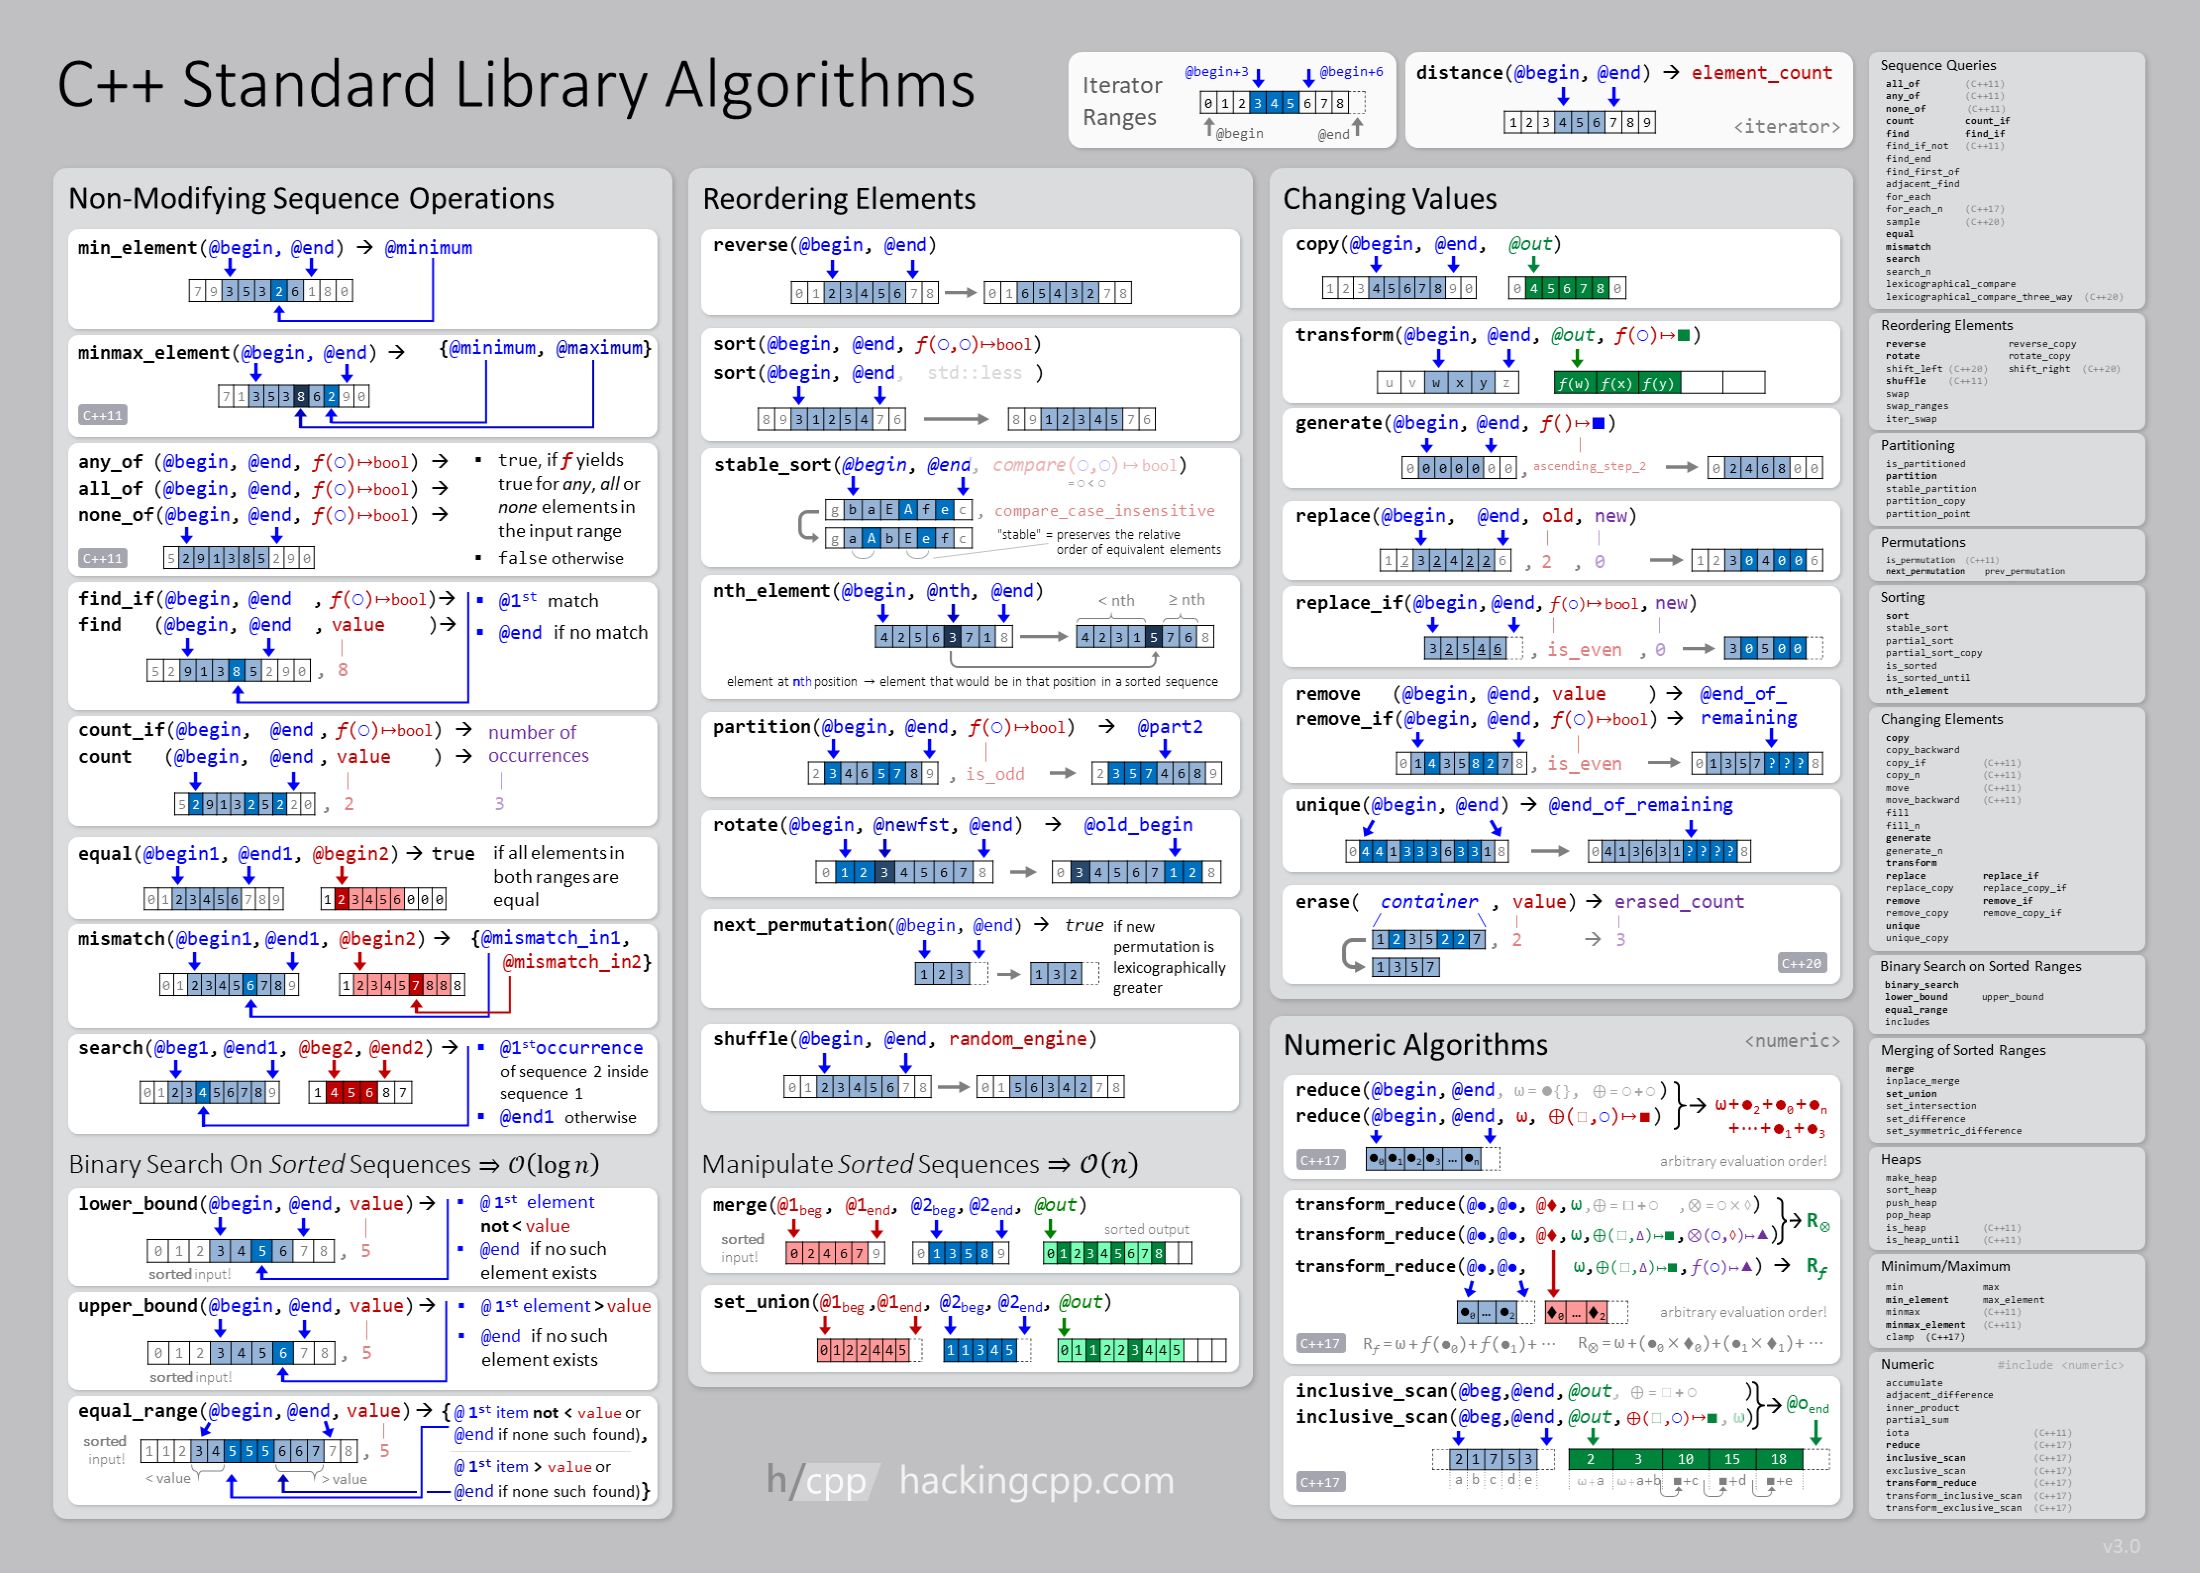
\includegraphics[width=1.2\textwidth, height=1.2\textheight, keepaspectratio]{./imgs/Algorithm_Library/algorithms.png}
	\caption{Algorithm Library}
	\label{fig:algorithms}
\end{figure}

% ------------------ SECTION: OPERAZIONI SU SEQUENZE NON-MODIFICABILI  ---------------

\newpage

\section{Operazioni su sequenze non-modificabili}

\textsf{\small \textbf{Definizione: } Le \textbf{operazioni su sequenze non-modificabili}, da come si intende sono quelle operazioni che non modificano la sequenza, ma che attuano, compiono ricerche per trovare determinati elementi, contano gli elementi, testano varie condizioni, eccetera..} \\

\subsection{Condizioni}

\textsf{\small Possiamo testare se degli elementi sono presenti o no attraverso queste funzioni: \textbf{std::all\_of}, \textbf{std::any\_of}, \textbf{std::none\_of}.} \\

\begin{itemize}
	\item \textsf{\small \textbf{any\_of} : ha bisogno che anche solo 1 sia vero (sia presente).}
	\item \textsf{\small \textbf{all\_of} : ha bisogno che tutti quelli considerati siano veri.}
	\item \textsf{\small \textbf{none\_of} : ha bisogno che nessuno sia presente (tra quelli cercati) (che siano tutti falsi).}
\end{itemize}

\begin{lstlisting}
	#include <iostream>
	#include <vector>
	#include <algorithm>
	
	int main()
	{
		std::vector<int> a = { 6, 1, 7, 3, 2, 5, 4, 9, 12 };
		std::vector<int> b = { 1, 4, 5, 8, 21, 11, 7, 0, 17 };
		
		// Ci assicuriamo che ci sia almeno un valore minore o uguale a 3 nel vettore a.
		std::cout << std::boolalpha << std::any_of( a.cbegin(), a.cend(), [](auto n) {return n <= 3; }) << "\n"; //Output: true
		
		// Ci assicuriamo che non ci siano valori maggiori di 33 nel vettore b.
		std::cout << std::boolalpha << std::none_of( b.cbegin(), b.cend(), [](auto n) { return n > 33; }) << "\n"; //Output: true
		
		std::vector<int> c = {0, 2, 4, 6, 8, 10};
		
		// Controlliamo se tutti i valori sono pari.
		if(std::all_of(c.cbegin(), c.cend(), [](int i){ return i % 2 == 0;}))
		{
			std::cout << "Tutti i numeri sono pari" << "\n";
		}
	
		//Output: Tutti i numeri sono pari.
		
		return 0;
	}	
\end{lstlisting}

\subsection{Ricerca}

\textsf{\small Queste operazioni servono per cercare degli elementi all'interno delle sequenze: \textbf{std::find}, \textbf{std::find\_if}, \textbf{std::find\_if\_not}, \textbf{find\_end}, \textbf{find\_first\_of}, \textbf{adjacent\_find}.} \\

\textsf{\small Inoltre ci sono anche: \textbf{std::search}, \textbf{search\_n}.} \\

\begin{lstlisting}
	#include <iostream>
	#include <string>
	#include <algorithm>
	#include <vector>
	
	int main()
	{
		// ESEMPIO FIND
		std::vector<std::string> a = { "zero", "one", "two", "three", "four", "five", "six", "seven", "eight", "nine", "ten" };
		std::vector<std::string> b = { "0", "1", "2", "3", "4", "5", "6", "7", "8", "9", "10" };
		
		// rbegin() e rend() servono per invertire (reverse) l'iteratore.
		const auto k = std::find( a.rbegin(), a.rend(), "one");
		std::cout << "Indice dell'ultimo 'one': " << (a.rend() - k) - 1 << std::endl; //Output: Indice dell'ultimo 'one': 1
		
		// ESEMPIO find\_first\_of
		const std::string s = "one;two,three:four";
		const std::string delimiter = ";,:";
		
		const auto i = std::find_first_of( s.cbegin(), s.cend(), delimiter.cbegin(), delimiter.cend());
		std::cout << "Indice del primo delimitatore: " << i - s.cbegin() << std::endl; //Output: Indice del primo delimitatore: 3
		
		// ESEMPIO adjacent\_find
		const std::string haystack = "as55jsdjflkadfkjsadlfs5j";
		const std::string needle = "s5j";
		
		const auto j = std::adjacent_find( haystack.cbegin(), haystack.cend() );
		std::cout << j - haystack.cbegin() << std::endl; //Output: 2
		
		// ESEMPIO SEARCH
		// Cerchiamo una sequenza nella stringa.
		const auto w = std::search( haystack.begin(), haystack.end(), needle.begin(), needle.end());
		std::cout << w - haystack.begin() << std::endl; //Output: 21
		return 0;
	}
\end{lstlisting}

\textsf{\small Questi sono alcuni esempi dell'utilizzo di questi funzioni, non li faccio tutti, ma gli altri sono intuitivi.} \\

\subsubsection{find vs search}

\textsf{\small La differenza è che \textbf{find} cerca un singolo elemento nella sequenza, mentre \textbf{search} cerca per un'intera sequenza nella sequenza. } \\

\subsection{Contatori}

\textsf{\small Ci sono un paio di funzioni per contare gli elementi di una sequenza: \textbf{std::count}, \textbf{std::count\_if}.} \\

\begin{lstlisting}
	#include <iostream>
	#include <algorithm>
	#include <vector>
	
	int main()
	{
		std::vector<int> v = { 8, 4, 9, 2, 3, 6, 5, 5, 1, 2, 4, 9, 1, 2};
		
		std::cout << std::count( v.begin(), v.end(), 3) << std::endl; //Output: 1
		
		std::cout << std::count_if( v.begin(), v.end(), [](auto n) { return n <= 7;}) << std::endl; //Output: 11
		return 0;
	}
\end{lstlisting}

\subsection{Altre operazioni}

\textsf{\small Ulteriori operazioni possibili sono: } \\

\begin{itemize}
	\item \textsf{\small \textbf{mismatch} : restituisce la prima posizione in cui due sequenze differiscono.}
	\item \textsf{\small \textbf{equal} : per controllare se due sequenze sono uguali (lo tratterò anche nelle \emph{Operazioni di Comparazione}).}
	\item \textsf{\small \textbf{is\_permutation} : testa se la sequenza è una permutazione (lo tratterò anche nelle \emph{Operazioni di Permutazione}).}
\end{itemize}

\begin{lstlisting}
	#include <iostream>
	#include <algorithm>
	#include <vector>
	
	int main()
	{
		// ESEMPIO MISMATCH
		std::vector<std::string> a = { "0", "1", "2", "3", "4", "5", "6", "7", "8", "9", "10" };
		std::vector<std::string> b = { "0", "1", "2", "3", "4", "&", "6", "7", "8", "9", "10" };
		
		const auto i = std::mismatch( a.cbegin(), a.cend(), b.cbegin()).first;
		std::cout << i - a.cbegin() << std::endl; //Output: 5
		
		// ESEMPIO EQUAL
		std::vector<int> v1 = { 1, 2, 3, 4, 5, 6 };
		std::vector<int> v2 = { 1, 2, 3, 4, 5, 6 };
		std::vector<int> v3 = { 1, 2, 4, 3, 5, 6 };
		
		std::cout << std::boolalpha << std::equal( v1.cbegin(), v1.cend(), v2.cbegin()) << std::endl; //Output: true
		std::cout << std::boolalpha << std::equal( v1.cbegin(), v1.cend(), v3.cbegin()) << std::endl; //Output: false
		
		// ESEMPIO IS\_PERMUTATION
		std::vector<int> vec = { 1, 2, 3, 4 };
		std::vector<int> vec2 = { 2, 3, 4, 1 };
		std::vector<int> vec3 = { 2, 3, 2, 2 };
		
		std::cout << std::boolalpha << std::is_permutation(vec.begin(), vec.end(), vec2.begin()) << std::endl; //Output: true
		std::cout << std::boolalpha << std::is_permutation(vec.begin(), vec.end(), vec3.begin()) << std::endl; //Output: false
		return 0;
	}
\end{lstlisting}

\fleuron %TODO: oppure \ornament

\textsf{\small Per tutte queste operazioni c'è un equivalente per \emph{ranges} del C++20 a pag. \pageref{ranges_seq_non_modificabili}} \\

% ------------------ SECTION: OPERAZIONI SU SEQUENZE MODIFICABILI --------------------

\newpage

\section{Operazioni su sequenze modificabili}

\textsf{\small \textbf{Definizione: } Queste, invece sono quelle operazioni che ti permettono di modificare la sequenza originaria.} \\

\subsection{Copiare sequenze | Copy}

\textsf{\small Queste operazioni ti permettono di copiare parti o intere sequenze: \textbf{std::copy}, \textbf{std::copy\_n}, \textbf{std::copy\_if}, \textbf{std::copy\_backward}.} \\

\begin{lstlisting}
	#include <iostream>
	#include <algorithm>
	#include <vector>
	#include <string>
	#include <iterator> // per usare gli iteratori nei loops.
	#include <cctype> // per usare std::isupper.
	
	int main()
	{
		// ESEMPIO COPY\_N
		std::vector<std::string> b = { "0", "1", "2", "3", "4", "5", "6", "7", "8", "9", "10" };
		
		std::vector<std::string> c;
		
		c.resize(9);
		
		std::copy_n( b.begin(), 9, c.begin());
		
		// A sto giro devo usare begin() ed end(), non posso usare cbegin() e cend().
		std::cout << "il vettore c contiene: ";
		for (std::vector<std::string>::iterator it = c.begin(); it!=c.end(); ++it)
		{
			std::cout << ' ' << *it;
		}
	
		std::cout << '\n';
	
		//Output: il vettore c contiene: 0 1 2 3 4 5 6 7 8
		
		// ESEMPIO COPY\_N 2
		std::string in = "1234567890";
		std::string out;
		
		std::copy_n(in.begin(), 4, std::back_inserter(out));
		std::cout << out << '\n'; //Output: 1234
		
		// ESEMPIO COPY\_IF
		std::string a = "Solo Le Lettere in Maiuscolo Verranno Considerate";
		
		std::string uppers;
		
		// back\_inserter è uno speciale tipo di \emph{output iterator} per 
		// permettere agli algoritmi che sovrascrivono gli elementi, come il 
		// \emph{copy} di inserire in dei nuovi elementi automaticamente alla fine del container.
		std::copy_if(a.begin(), a.end(), std::back_inserter( uppers ), [](auto s){ return std::isupper(s); } ); // una volta funzionava anche così: std::copy\_if(a.begin(), a.end(), std::back\_inserter( uppers), std::isupper);
		std::cout << uppers << std::endl; //Output: SLLMVC
		
		// ESEMPIO COPY\_BACKWARD
		std::vector<int> inVector;
		for(int i = 0; i < 10; i++)
		{
			inVector.push_back(i);
		}
	
		std::vector<int> outVector(15);
		
		std::copy_backward(inVector.begin(), inVector.end(), outVector.end());
		
		std::cout << "outVector contiene: ";
		for(auto v : outVector){
			std::cout << v << " ";
		}
	
		//Output: outVector contiene: 0 0 0 0 0 0 1 2 3 4 5 6 7 8 9
		return 0;
	}
\end{lstlisting}

\subsection{Muovere | Move}

\textsf{\small Queste ci permettono di spostare gli elementi da una sequenza ad un'altra: \textbf{std::move}, \textbf{std::move\_backward}.} \\

\begin{lstlisting}
	#include <iostream>
	#include <vector>
	#include <string>
	#include <algorithm>
	
	int main()
	{
		std::vector<std::string> a = { "zero", "one", "two", "three", "four", "five", "six", "seven", "eight", "nine", "ten" };
		std::vector<std::string> b = { "0", "1", "2", "3", "4", "&", "6", "7", "8", "9", "10" };
		
		// Sposta i primi due parametri di move nell'inizio del suo terzo parametro.
		std::move( a.begin(), a.begin() + 3, b.begin()); // anche mettendo a.begin() funziona.
		
		std::cout << "il vettore a contiene: ";
		for(auto v : a){
			std::cout << v << " ";
		}
	
		//Output: Il vettore a contiene: three four five six seven eight nine ten
		
		return 0;
	}
\end{lstlisting}

\subsection{Scambiare | Swap}

\textsf{\small Le operazioni di \textbf{swap} ci permettono di scambiare gli elementi di due sequenze, contenitore: \textbf{std::swap}, \textbf{std::swap\_ranges}, \textbf{iter\_swap}.} \\

\begin{lstlisting}
	#include <iostream>
	#include <algorithm>
	#include <vector>
	
	int main()
	{
		// ESEMPIO SWAP
		int x = 5, int y = 12;
		
		std::cout << "x prima dello swap: " << x << ", y prima dello swap: " << y << std::endl; //Output: x prima dello swap: 5, y prima dello swap: 12
		
		std::swap(x,y);
		
		std::cout << "x dopo lo swap: " << x << ", y dopo lo swap: " << y << std::endl; //Output: x dopo lo swap: 12, y dopo lo swap: 5
		
		//ESEMPIO SWAP\_RANGES
		std::vector<int> vec1(7, 66);
		std::vector<int> vec2(7, 18);
		
		std::swap_ranges(vec1.begin() + 1, vec1.end() - 1, vec2.begin());
		
		std::cout << "vec1 contiene: ";
		for(auto v : vec1){
			std::cout << v << " ";
		}
	
		//Output: vec1 contiene: 66 18 18 18 18 18 66
		
		std::cout << '\n';
		
		std::cout << "vec2 contiene: ";
		for(auto v : vec2){
			std::cout << v << " ";
		}
	
		//Output: vec2 contiene: 66 66 66 66 66 18 18
		
		std::cout << '\n';
		return 0;
	}
\end{lstlisting}

\subsection{Trasformare | Transform}

\textsf{\small Applica un'operazione sugli elementi delle sequenze: \textbf{std::transform}.} \\

\textsf{\small \textbf{In Place} : vuol dire che il risultato viene messo nello stesso contenitore non in un altro a parte.} \\

\begin{lstlisting}
	#include <iostream>
	#include <algorithm>
	#include <vector>
	#include <cctype>
	
	int main()
	{
		// ESEMPIO 1
		std::vector<int> a = { 5, 7, 8, 9, 1, 2};
		std::vector<int> b = { 3, 6, 2, 1, 0, 9};
		
		std::vector<int> c;
		
		std::transform( a.begin(), a.end(), b.begin(), std::back_inserter(c), [](int a, int b) { return a + b * b; });
		
		std::cout << "c contiene: ";
		for(auto v : c)
		{
			std::cout << v << " ";
		}
		
		std::cout << '\n';
		
		//Output: c contiene: 14 43 12 10 1 83
		
		//ESEMPIO 2
		std::string s = "Questa frase verra\' trasformata";
		std::string out;
		
		std::transform( s.begin(), s.end(), std::back_inserter(out), [](auto o){return std::toupper(o);});
		
		std::cout << out << '\n';
		
		//Output: QUESTA FRASE VERRA' TRASFORMATA
		return 0;
	}
\end{lstlisting}

\subsection{Rimpiazzare | Replace}

\textsf{\small Queste permettono di rimpiazzare alcuni elementi della sequenza con altri: \textbf{std::replace}, \textbf{std::replace\_if}, \textbf{std::replace\_copy}, \textbf{std::replace\_copy\_if}.} \\

\begin{lstlisting}
	#include <iostream> // per std::cout
	#include <algorithm> // per std::replace, replace\_if, replace\_copy\_if
	#include <vector> // per std::vector
	#include <array> // per std::array
	#include <iterator> // per std::ostream\_iterator
	#include <functional> // per std::bind
	
	int main()
	{
		// ESEMPIO REPLACE
		std::array<int, 10> arr{3, 2, 1, 7, 8, 6, 11, 9, 0, 33};
		
		std::replace(arr.begin(), arr.end(), 6, 66);
		
		for (int a : arr) {
			std::cout << a << " ";
		}
		std::cout << '\n';
		
		//Output: 3 2 1 7 8 66 11 9 0 33
		
		// ESEMPIO REPLACE\_IF
		// Se è minore di 3 allora lo sostituiamo con 37.
		std::replace_if(arr.begin(), arr.end(), 
		std::bind(std::less<int>(), std::placeholders::_1, 3), 37);
		for (int a : arr) {
			std::cout << a << " ";
		}
		std::cout << '\n';
		
		//Output: 3 37 37 7 8 66 11 9 37 33
		
		// ESEMPIO REPLACE\_COPY\_IF
		std::vector<int> v{6, 1, 22, 66, 3, 9, 8, 1, 4, 5, 7, 0 };
		std::replace_copy_if(v.begin(), v.end(), std::ostream_iterator<int>(std::cout, " "), [](int n) { return n > 6; }, 33);
		std::cout << '\n';
		
		//Output: 6 1 33 33 3 33 33 1 4 5 33 0
		return 0;
	}
\end{lstlisting}

\subsection{Riempire | Fill}

\textsf{\small Utilizziamo \textbf{std::fill} e \textbf{std::fill\_n} per riempire una sequenza con una serie di elementi.} \\

\begin{lstlisting}
	#include <iostream>
	#include <algorithm>
	#include <vector>
	#include <iterator>
	
	int main()
	{
		std::vector<int> v(10, 21);
		v.reserve(10);
		std::fill_n( std::back_inserter( v ), 10, 36);
		
		for(auto e : v)
		{
			std::cout << e << " ";
		}
	
		std::cout << '\n';
		
		//Output: 21 21 21 21 21 21 21 21 21 21 36 36 36 36 36 36 36 36 36 36
		return 0;
	}
\end{lstlisting}

\subsection{Generatori | Generate}

\textsf{\small Servono per generare elementi in base ad una funzione generatrice. Questa è definita dall'utente ed è chiamata in modo successivo per assegnare gli elementi, numeri. Queste sono: \textbf{std::generate}, \textbf{std::generate\_n}. } \\

\begin{lstlisting}
	#include <iostream>
	#include <algorithm>
	#include <vector>
	#include <iterator>
	#include <random>
	#include <functional>
	
	int main()
	{
		// ESEMPIO 1
		std::vector<int> v;
		std::generate_n( std::back_inserter(v), 8, [val = 0]() mutable {
			const auto old = val;
			val += 6;
			return old;
		});
	
		for(auto e : v)
		{
			std::cout << e << " ";
		}
		
		std::cout << '\n';
	
		//Output: 0 6 12 18 24 30 36 42
	
		// ESEMPIO 2
		std::vector<int> v2;
		
		std::mt19937 rng( std::random_device{}() );
		std::uniform_int_distribution<int> d(0, 20);
		
		std::generate_n( std::back_inserter(v2), 8, std::bind(d, rng));
		
		for(auto e : v2)
		{
			std::cout << e << " ";
		}
		
		std::cout << '\n';
		
		//Output: 9 6 15 19 14 3 13 8 (pseudo-casuale ogni volta)
		return 0;
	}
\end{lstlisting}

%TODO: generate vs fill (direi non necessario)

\subsection{Rimozione | Remove}

\textsf{\small Come implica dal nome, queste operazioni forniscono un modo per rimuovere elementi da una sequenza: \textbf{std::remove}, \textbf{std::remove\_if}, \textbf{std::remove\_copy}, \textbf{std::remove\_copy\_if}.} \\

\begin{lstlisting}
	#include <iostream>
	#include <algorithm>
	#include <vector>
	#include <string>
	#include <cctype>
	
	int main()
	{
		std::string str = " Testo con degli   spazi bianchi";
		
		auto noSpace = std::remove(str.begin(), str.end(), ' ');
		
		std::cout << str << std::endl; //Output: Testocondeglispazibianchibianchi
		
		std::string str2 = "Testo\n con\tdegli   spazi bianchi\n\n";
		str2.erase(std::remove_if(str2.begin(), str2.end(), 
		[](unsigned char c){return std::isspace(c);}), str2.end());
		
		std::cout << str2 << std::endl; //Output: Testocondeglispazibianchi
		return 0;
	}
\end{lstlisting}

\subsection{Unico | Unique}

\textsf{\small Permettono di ottenere una sequenza unica, senza elementi ripetuti.} \\

\begin{lstlisting}
	#include <iostream>
	#include <algorithm>
	#include <vector>
	#include <string>
	#include <iterator>
	
	int main()
	{
		// ESEMPIO UNIQUE
		std::vector<std::string> s = { "0", "1", "2", "2", "2", "3", "5", "4", "6", "9", "9", "5", "11" };
		
		const auto s2 = std::unique(s.begin(), s.end());
		s.erase(s2, s.end());
		
		for(auto e : s)
		{
			std::cout << e << " ";
		}
		
		std::cout << '\n';
		//Output: 0 1 2 3 5 4 6 9 5 11
		
		// ESEMPIO UNIQUE\_COPY
		std::string str1 = "La      stringa    con molti       spazi   bianchi!";
		std::cout << "prima: " << str1 << '\n'; //Output: La      stringa    con molti       spazi   bianchi!
		
		std::string str2;
		std::unique_copy(str1.begin(), str1.end(), std::back_inserter(str2),
		[](char c1, char c2){ return c1 == ' ' && c2 == ' '; });
		
		std::cout << "dopo:  " << str2 << '\n'; //Output: La stringa con molti spazi bianchi!
		return 0;
	}
\end{lstlisting}

\subsection{Invertire | Reverse}

\textsf{\small Queste operazioni consentono di invertire l'ordine delle sequenze: \textbf{std::reverse}, \textbf{std::reverse\_copy}.} \\

\begin{lstlisting}
	#include <iostream>
	#include <algorithm>
	#include <vector>
	
	int main()
	{
		// ESEMPIO REVERSE
		std::vector<int> vec{ 9, 6, 3};
		std::reverse(vec.begin(), vec.end());
		for(auto v : vec) std::cout << v;
		std::cout << '\n';
		//Output: 369
		
		// ESEMPIO REVERSE\_COPY
		std::vector<int> vec2({2, 1, 4});
		
		std::vector<int> reverseVec(3);
		
		std::reverse_copy(std::begin(vec2), std::end(vec2), std::begin(reverseVec));
		for(auto v : reverseVec)
		{
			std::cout << v << " ";
		}
	
		std::cout << '\n';
		//Output: 4 1 2
		return 0;
	}
\end{lstlisting}

\subsection{Ruotare | Rotate}

\textsf{\small Ruotano l'ordine degli elementi nella sequenza: \textbf{std::rotate}, \textbf{std::rotate\_copy}.} \\

\begin{lstlisting}
	#include <iostream>
	#include <algorithm>
	#include <vector>
	
	int main()
	{
		std::vector<int> v{3, 7, 9, 8, 2, 1, 0, 10, 4, 5, 12};
		
		// Rotazione verso sinistra
		std::rotate(v.begin(), v.begin() + 1, v.end());
		
		for(auto e : v) std::cout << e << " ";
		std::cout << '\n';
		
		//Output: 7 9 8 2 1 0 10 4 5 12 3
		
		// Rotazione verso destra
		std::rotate(v.rbegin(), v.rbegin() + 1, v.rend());
		
		for(auto e : v) std::cout << e << " ";
		std::cout << '\n';
		
		//Output: 3 7 9 8 2 1 0 10 4 5 12
		return 0;
	}
\end{lstlisting}

\subsection{Spostare | Shift}

\textsf{\small Servono per spostare di tot elementi le sequenze, a differenza della rotazione che si limita a ruotare la sequenza, con lo spostamento si perdono o si ottengono dati.} \\

\begin{lstlisting}
	#include <iostream>
	#include <algorithm>
	#include <vector>
	#include <string>
	
	int main()
	{
		std::vector<std::string>  g{"a", "b", "c", "d", "e", "f", "g"};
		
		std::shift_left( begin(g), end(g), 3 );
		
		for(auto s : g) std::cout << s << " ";
		std::cout << '\n';
		
		//Output: . . . d e f g (in realtà mi dava errore std::shift\_left non è membro di std)
		
		std::shift_right( begin(g), end(g), 3);
		for(auto s : g) std::cout << s << " ";
		std::cout << '\n';
		
		//Output: . . . d . . . (in realtà mi dava errore std::shift\_right non è membro di std)
		
		return 0;
	}
\end{lstlisting}

\subsection{Mischiare | Shuffle}

\textsf{\small Serve per mischiare, mescolare gli elementi della sequenza: \textbf{std::shuffle}, \textbf{std::random\_shuffle}.} \\

\begin{lstlisting}
	#include <iostream>
	#include <algorithm>
	#include <vector>
	#include <string>
	#include <random>
	
	int main()
	{
		std::vector<std::string> a = { "zero", "one", "two", "three", "four", "five", "six", "seven", "eight", "nine", "ten" };
		
		std::mt19937 rng( std::random_device{}());
		std::shuffle( a.begin(), a.end(), rng );
		
		for(auto s : a) std::cout << s << " ";
		std::cout << '\n';
		
		//Output: three zero four two ten one nine seven six eight five (è sempre diversa perché è casuale)
		return 0;
	}
\end{lstlisting}

\fleuron

\textsf{\small Per tutte queste operazioni c'è un equivalente per \emph{ranges} del C++20 a pag. \pageref{ranges_seq_modificabili}} \\

% ---------------------- SECTION: OPERAZIONI SU PARTIZIONI ---------------------------

\section{Operazioni su Partizioni}

\textsf{\small \textbf{Definizione: } Le \textbf{operazioni su partizioni} permettono di eseguire partizioni sulle sequenze di elementi.} \\

\textsf{\small Queste operazioni possibili sono: \textbf{std::partition}, \textbf{std::is\_partitioned}, \textbf{std::stable\_partition}, \textbf{std::partition\_copy}, \textbf{std::partition\_point}.} \\

\begin{lstlisting}
	#include <iostream>
	#include <algorithm>
	#include <vector>
	#include <array>
	
	int main()
	{
		// ESEMPIO PARTITION
		std::vector<std::string> a = { "zero", "one", "two", "three", "four", "five", "six", "seven", "eight", "nine", "ten" };
		std::vector<int> b = {0, 1, 2, 3, 4, 5, 6, 7, 8, 9, 10};
		
		auto partion1 = std::partition( a.begin(), a.end(), [](const auto& s) { return std::any_of( s.begin(), s.end(), []( char c){ return c == 'e'; });});
		
		for(auto p : a)
		{
			std::cout << p << " ";
		}
	
		std::cout << '\n';
		
		//Output: zero one ten three nine five eight seven six four two
		
		auto partition2 = std::partition( b.begin(), b.end(), [](int i) { return i % 2 == 0;});
		
		for(auto p : b)
		{
			std::cout << p << " ";
		}
		
		std::cout << '\n';
		
		//Output: 0 10 2 8 4 6 5 7 3 9 1
		
		// ESEMPIO STABLE\_PARTITION
		std::vector<std::string> c = { "zero", "one", "two", "three", "four", "five", "six", "seven", "eight", "nine", "ten" };
		std::vector<int> d = {0, 1, 2, 3, 4, 5, 6, 7, 8, 9, 10};
		
		auto partion3 = std::stable_partition( a.begin(), a.end(), [](const auto& s) { return std::any_of( s.begin(), s.end(), []( char c){ return c == 'e'; });});
		
		for(auto p : c)
		{
			std::cout << p << " ";
		}
		
		std::cout << '\n';
		
		//Output: zero one two three four five six seven eight nine ten
		
		auto partition4 = std::stable_partition( b.begin(), b.end(), [](int i) { return i % 2 == 0;});
		
		for(auto p : d)
		{
			std::cout << p << " ";
		}
		
		std::cout << '\n';
		
		//Output: 0 1 2 3 4 5 6 7 8 9 10
		
		//ESEMPIO IS\_PARTITIONED
		std::vector<int> v = { 2, 4, 8, 6, 0, 10};
		bool isPartitioned = std::is_partitioned( v.begin(), v.end(), [](int i){ return i % 2 == 0; });
		
		std::cout << std::boolalpha << isPartitioned << std::endl; //Output: true
		
		// ESEMPIO PARTITION\_COPY
		int arr [10] = {1,2,3,4,5,6,7,8,9,10};
		int trueArr [5] = {0};
		int falseArr [5] = {0};
		
		std::partition_copy(std::begin(arr), std::end(arr), std::begin(trueArr), std::begin(falseArr), [](int i){return i > 5; });
		
		for(int a : trueArr)
		{
			std::cout << a << " ";
		}
		
		std::cout << '\n';
		
		//Output: 6 7 8 9 10
		
		for(int a : falseArr)
		{
			std::cout << a << " ";
		}
		
		std::cout << '\n';
		
		//Output: 1 2 3 4 5
		
		// ESEMPIO PARTITION\_POINT
		std::array v = { 1, 2, 3, 4, 5, 6, 7, 8, 9 };
		auto is_even = [](int i){ return i % 2 == 0; };
		const auto parPoint = std::partition_point(v.cbegin(), v.cend(), is_even);
		const auto i = std::distance(v.cbegin(), pp);
		std::cout << "Partition point a: " << i << "; v[" << i << "] = " << *pp << '\n'; //Output: Partition point a: 4; v[4] = 5
		return 0;
	}
\end{lstlisting}

\fleuron

\textsf{\small Per tutte queste operazioni c'è un equivalente per \emph{ranges} del C++20 a pag. \pageref{ranges_partition}} \\

% --------------------- SECTION: OPERAZIONI DI ORDINAMENTO ---------------------------

\newpage

\section{Operazioni di Ordinamento}

\textsf{\small \textbf{Definizione: } Le \textbf{operazioni di ordinamento} consentono di ordinare le sequenze.} \\

\textsf{\small Queste sono: \textbf{std::sort}, \textbf{std::stable\_sort}, \textbf{std::partial\_sort}, \textbf{std::partial\_sort\_copy}, \textbf{std::is\_sorted}, \textbf{std::is\_sorted\_until}, \textbf{std::nth\_elemeent}.} \\

\begin{lstlisting}
	#include <iostream>
	#include <algorithm>
	#include <vector>
	#include <string>
	
	int main()
	{
		// ESEMPIO SORT E IS\_SORTED
		std::vector<int> v{ 7, 9, 1, 0, 2, 5, 3, 4, 8, 10, 6};
		
		std::cout << std::boolalpha << std::is_sorted(v.begin(), v.end()) << '\n'; //Output: false
		
		std::sort(v.begin(), v.end());
		
		for(auto e : v)
		{
			std::cout << e << " ";
		}
	
		std::cout << '\n';
		
		//Output: 0 1 2 3 4 5 6 7 8 9 10
		
		std::cout << std::boolalpha << std::is_sorted(v.begin(), v.end()) << '\n'; //Output: true
		
		// ESEMPIO SORT 
		// Il sort, di solito usa il minore < per fare l'ordinamento, ma in questo caso noi gli passiamo il maggiore >.
		std::sort(v.begin(), v.end(), std::greater<int>{});
		
		for(auto e : v)
		{
			std::cout << e << " ";
		}
		
		std::cout << '\n';
		
		//Output: 10 9 8 7 6 5 4 3 2 1 0
		
		// ESEMPIO STABLE\_SORT
		class Employee {
			public:
				int age;
				std::string name;  // Non partecipa nei paragoni
		};
		
		// Questo ci serve per indicare alle funzioni sort come devono fare il paragone per ordinare gli elementi.
		bool operator<(const Employee & lhs, const Employee & rhs)
		{
			return lhs.age < rhs.age;
		}
	
		std::vector<Employee> employees =
		{ 
			{22, "Gigi"},
			{37, "Maria"},
			{48, "Alessio"},
		};
	
		std::stable_sort(v.begin(), v.end());
		
		for (const Employee & e : employees)
			std::cout << e.age << ", " << e.name << '\n';
			
		//Output: 22, Gigi
		//Output: 37, Maria
		//Output: 48, Alessio
		
		// ESEMPIO PARTIAL\_SORT
		std::vector<int> v2 = { 5, 7, 1, 0, 3, 5, 6, 4, 7, 8, 10, 2 };
		
		// Ordina solo una parte del contenitore, non tutto.
		// Può essere utile, magari per delle classifiche, dove magari servono soltanto i primi 10 o i primi 100 giocatori e non tutti gli altri.
		std::partial_sort(v2.begin(), v2.begin() + 4, v2.end());
		
		for(auto& v : v2)
		{
			std::cout << v << " ";
		}
	
		std::cout << '\n';
		
		//Output: 0 1 2 3 7 5 6 5 7 8 10 4 (i primi 4 elementi sono ordinati: 0 1 2 3, tutti gli altri son rimasti in posizioni non ordinate)
		
		// ESEMPIO NTH\_ELEMENT
		std::vector<int> v3{11, 7, 9, 4, 2, 2, 6, 7, 9, 3, 7, 7};
		
		auto m = v3.begin() + v3.size()/2;
		std::nth_element(v3.begin(), m, v3.end());
		
		for(auto& e : v3)
		{
			std::cout << e << " ";
		}
		
		std::cout << '\n';
		
		//Output: 6 2 3 4 2 7 7 7 9 9 7 11
		
		std::cout << "The medianIl mediano è: " << v3[v3.size()/2] << '\n'; //Output: Il mediano è 7
		
		return 0;
	}
\end{lstlisting}

\fleuron

\textsf{\small Per tutte queste operazioni c'è un equivalente per \emph{ranges} del C++20 a pag. \pageref{ranges_sorting}} \\

% ------------ SECTION: OPERAZIONI DI RICERCA BINARIA (BINARY SEARCH) ----------------

\newpage

\section{Operazioni di Ricerca Binaria}

\textsf{\small \textbf{Definizione: } Queste servono per operazioni su ricerche binarie: \textbf{std::lower\_bound}, \textbf{std::upper\_bound}, \textbf{std::equal\_range}, \textbf{std::binary\_search}.} \\

\begin{lstlisting}
	#include <iostream>
	#include <algorithm>
	#include <vector>
	
	int main()
	{
		// ESEMPIO LOWER\_BOUND
		std::vector<int> v{ 15, 5, 22, 11, 33, 7, 88, 0, 9, 1, 4, 26, 52 };
		
		// Restituisce un iteratore che punta al primo elemento che non è minore del valore.
		const int lowerBound = 3;
		const auto i = std::lower_bound(v.begin(), v.end(), lowerBound);
		
		std::cout << *i << '\n'; //Output: 15
		
		// ESEMPIO UPPER\_BOUND
		// Restituisce un iteratore che punta al primo elemento che è maggiore del valore.
		const int upperBound = 7;
		const auto j = std::upper_bound(v.begin(), v.end(), upperBound);
		
		std::cout << *j << '\n'; //Output: 22
		
		// ESEMPIO EQUAL\_RANGE
		std::vector<int> v = { 11, 10, 33, 33, 33, 111, 10,
			333, 369, 77, 77, 80 };
		
		// Dichiariamo un iteratore per il
		// valore di ritorno di std::equal\_range
		std::pair<std::vector<int>::iterator,
		std::vector<int>::iterator> it;
		
		std::sort(v.begin(), v.end());
		// v diventa 10 10 11 33 33 33 77 77 80 111 333 369
		
		// Usiamo std::equal\_range e compariamo gli elementi
		// con 33
		it = std::equal_range(v.begin(), v.begin() + 12, 33);
		
		// Displaying the subrange bounds
		std::cout << "33 è presente nel vettore dall'indice: "
		<< (it.first - v.begin()) << " fino a: "
		<< (it.second - v.begin());
		
		//Output: 33 è presente nel vettore dall'indice: 3 fino a: 6
		
		// ESEMPIO BINARY\_SEARCH
		std::vector<int> haystack {1, 3, 7, 5, 9};
		std::vector<int> needles {7, 2, 3};
		
		for (auto needle : needles) {
			std::cout << "Cerco il: " << needle << '\n';
			if (std::binary_search(haystack.begin(), haystack.end(), needle)) {
				std::cout << "Trovato " << needle << '\n';
			} else {
				std::cout << "Non trovato!\n";
			}
		}
	
		//Output: Cerco il: 7
		//Output: Trovato
		//Output: Cerco il: 2
		//Output: Non trovato!
		//Output: Cerco il: 3
		//Output: Trovato
		
		return 0;
	}
\end{lstlisting}

\fleuron

\textsf{\small Per tutte queste operazioni c'è un equivalente per \emph{ranges} del C++20 a pag. \pageref{ranges_binary_search}} \\

% --------------- SECTION: ALTRE OPERAZIONI DI ORDINAMENTO SUI RANGES ----------------

%TODO: questa parte nella sezione sul C++20

% -------------------------- SECTION: OPERAZIONI DI MERGE ----------------------------

\newpage

\section{Operazioni di Fusione | Merge}

\textsf{\small \textbf{Definizione: } Le \textbf{operazioni di merge} permettono di combinare, di fondere gli elementi di due sequenze: \textbf{std::merge}, \textbf{std::inplace\_merge}.} \\

\begin{lstlisting}
	#include <iostream>
	#include <algorithm>
	#include <vector>
	#include <random>
	#include <functional>
	
	int main()
	{
		// ESEMPIO MERGE
		std::random_device rd;
		std::mt19937 mt(rd());
		std::uniform_int_distribution<> distribution(0, 9);
		
		std::vector<int> v1(10), v2(10);
		std::generate(v1.begin(), v1.end(), std::bind(distribution, std::ref(mt)));
		std::generate(v2.begin(), v2.end(), std::bind(distribution, std::ref(mt)));
		
		std::cout << "Prima del sorting" << '\n';
		
		for(auto& v : v1)
		{
			std::cout << v << " ";
		}
		std::cout << '\n';
		
		for(auto& v : v2)
		{
			std::cout << v << " ";
		}
		std::cout << '\n';
		
		//Output: Prima del sorting
		//Output: 5 6 1 8 4 9 2 5 2 2 (numeri generati casualmente)
		//Output: 6 0 6 5 7 8 8 2 8 5 (numeri generati casualmente)
		
		std::sort(v1.begin(), v1.end());
		std::sort(v2.begin(), v2.end());
		
		std::cout << "Dopo il sorting" << '\n';
		
		for(auto& v : v1)
		{
			std::cout << v << " ";
		}
		std::cout << '\n';
		
		for(auto& v : v2)
		{
			std::cout << v << " ";
		}
		std::cout << '\n';
		
		//Output: Dopo il sorting
		//Output: 1 2 2 2 4 5 5 6 8 9 
		//Output: 0 2 5 5 6 6 7 8 8 8
		
		std::vector<int> v3;
		std::merge(v1.begin(), v1.end(), v2.begin(), v2.end(), std::back_inserter(v3));
		
		std::cout << "v3 contiene: ";
		
		for(auto& v : v3)
		{
			std::cout << v << " ";
		}
		std::cout << '\n';
		
		//Output: v3 contiene: 0 1 2 2 2 2 4 5 5 5 5 6 6 6 7 8 8 8 8 9 (numeri generati casualmente)
		
		// ESEMPIO INPLACE\_MERGE
		int first[] = {7, 36, 12, 24, 8};
		int second[] = {57, 94, 14, 67, 80};
		
		std::vector<int> v(10);
		
		std::vector<int>::iterator it;
		
		std::sort (first,first+5);
		std::sort (second,second+5);
		
		it = std::copy (first, first+5, v.begin()); 
		std::copy (second,second+5,it);
		
		std::inplace_merge (v.begin(),v.begin()+5,v.end());
		
		std::cout << "Il vettore risultante contiene: ";
		for (it=v.begin(); it!=v.end(); ++it)
		{
			std::cout << ' ' << *it; 
		}
		std::cout << '\n';
		
		//Output: Il vettore risultante contiene:  7 8 12 14 24 36 57 67 80 94
		return 0;
	}
\end{lstlisting}

\fleuron

\textsf{\small Per tutte queste operazioni c'è un equivalente per \emph{ranges} del C++20 a pag. \pageref{ranges_merge}} \\

% ------------------------ SECTION: OPERAZIONI SUGLI INSIEMI -------------------------

\newpage

\section{Operazioni sugli Insiemi}

\textsf{\small \textbf{Definizione: } Le \textbf{operazioni sugli insiemi} permettono di attuare le tipiche operazioni matematiche: \emph{unione} : \textbf{std::set\_union}, \emph{intersezione} : \textbf{std::set\_intersection}, \emph{differenza} : \textbf{std::set\_difference}, \emph{simmetria differenza} : \textbf{std::set\_symmetric\_difference}.} \\

\begin{lstlisting}
	#include <iostream>
	#include <algorithm>
	#include <vector>
	#include <string>
	
	// Funzione per mostrare gli elementi di un std::vector
	template<typename T>
	void printVec(const std::vector<T>& v)
	{
		for(const auto& i : v)
		{
			std::cout << i << " ";
		}
		std::cout << '\n';
	}
	
	int main()
	{
		// ESEMPIO INCLUDES
		std::vector<char> v1 = { 'a', 'b', 'c', 'd', 'f', 'g' };
		std::vector<char> v2 = { 'a', 'b', 'c' };
		std::vector<char> v3 = { 'a', 'c' };
		
		printVec(v1);
		std::cout << "include: " << '\n';
		
		printVec(v2);
		
		std::cout << std::boolalpha << std::includes(v1.begin(), v1.end(), v2.begin(), v2.end()) << '\n'; //Output: true
		
		printVec(v3);
		
		std::cout << std::boolalpha << std::includes(v1.begin(), v1.end(), v3.begin(), v3.end()) << '\n'; //Output: false
		
		std::cout << std::flush;
		
		// ESEMPIO SET\_UNION, SET\_INTERSECTION, SET\_DIFFERENCE, SET\_SYMMETRIC\_DIFFERENCE
		std::vector<int> vec1{ 1, 2, 3, 5, 7, 9 };
		std::vector<int> vec2{ 6, 4, 1, 2, 3, 9, 11 };
		
		std::sort(vec1.begin(), vec1.end());
		std::sort(vec2.begin(), vec2.end());
		
		std::vector<int> destUnion;
		
		std::set_union(vec1.begin(), vec1.end(), vec2.begin(), vec2.end(), std::back_inserter(destUnion));
		
		std::cout << "unione: ";
		printVec(destUnion); //Output: unione: 1 2 3 4 5 6 7 9 11
		
		std::vector<int> destIntersection;
		
		std::set_intersection(vec1.begin(), vec1.end(), vec2.begin(), vec2.end(), std::back_inserter(destIntersection));
		
		std::cout << "intersezione: ";
		printVec(destIntersection); //Output: intersezione: 1 2 3 9
		
		std::vector<int> destDifference;
		
		std::set_difference(vec1.begin(), vec1.end(), vec2.begin(), vec2.end(), std::back_inserter(destDifference));
		
		std::cout << "differenza: ";
		printVec(destDifference); //Output: differenza: 5 7
		
		std::vector<int> destSymmDifference;
		
		std::set_symmetric_difference(vec1.begin(), vec1.end(), vec2.begin(), vec2.end(), std::back_inserter(destSymmDifference));
		
		std::cout << "differenza simmetrica: ";
		printVec(destSymmDifference); //Output: differenza simmetrica: 4 5 6 7 11 
		
		return 0;
	}
\end{lstlisting}

\fleuron

\textsf{\small Per tutte queste operazioni c'è un equivalente per \emph{ranges} del C++20 a pag. \pageref{ranges_set}} \\

% ------------------------- SECTION: OPERAZIONI SU HEAP ------------------------------

\newpage

\section{Operazioni su Heap}

\textsf{\small \textbf{Definizione: } L'\textbf{Heap} è una \emph{struttura dati} basata sugli \emph{alberi} che soddisfa la \textbf{proprietà degli heap}: } \\

\textsf{\small In un \textbf{max heap}: } \\

\begin{itemize}
	\item \textsf{\small le chiavi (il valore) di ciascun nodo padre son sempre maggiori o uguali a quelle dei nodi figli.}
	\item \textsf{\small La chiave (il valore) dal valore massimo appartiene alla radice (detta \emph{root node}).}
\end{itemize}

\textsf{\small In un \textbf{min heap}: } \\

\begin{itemize}
	\item \textsf{\small Le chiavi (il valore) di ciascun nodo sono minori o uguali a quelle dei figli.}
	\item \textsf{\small La chiave del valore minimo appartiene alla radice. }
\end{itemize}

\begin{figure}[H]
	\centering
	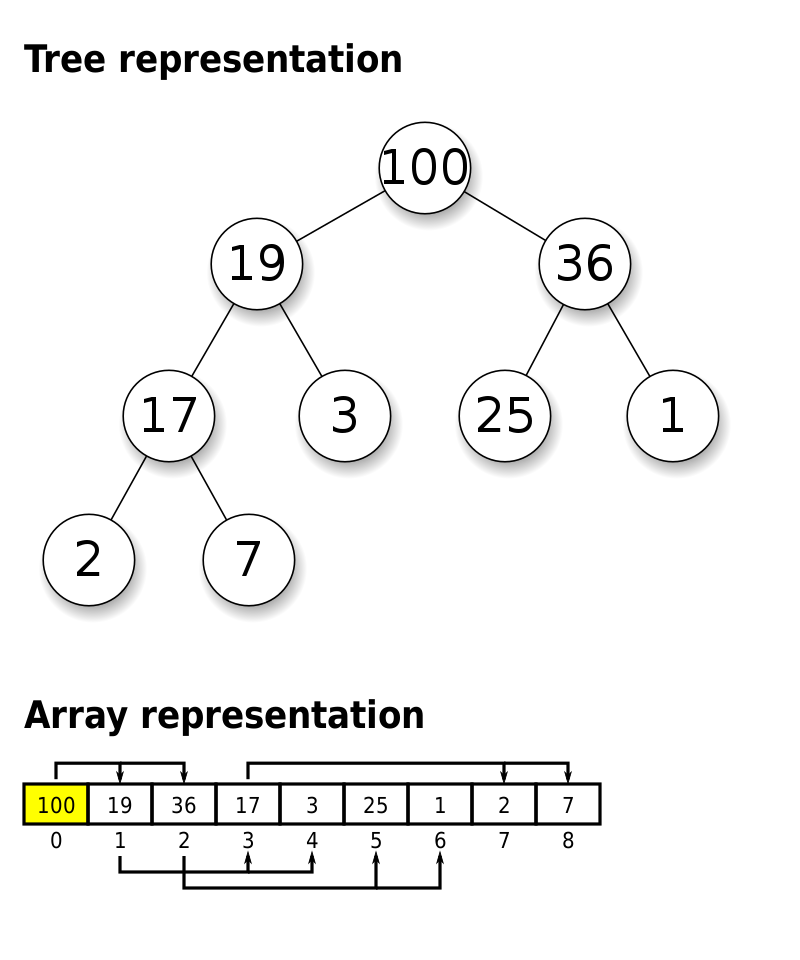
\includegraphics[width=1\textwidth, height=1\textheight, keepaspectratio]{./imgs/Algorithm_Library/Max-Heap.png}
	\caption{Max Heap}
	\label{fig:max-heap}
\end{figure}

\textsf{\small Le operazioni disponibili sugli heap sono: \textbf{std::push\_heap}, \textbf{std::pop\_heap}, \textbf{std::make\_heap}, \textbf{std::sort\_heap}, \textbf{std::is\_heap}, \textbf{std::is\_heap\_until}.} \\

\begin{lstlisting}
	#include <iostream>
	#include <algorithm>
	#include <vector>
	#include <random>
	#include <functional>
	
	// Funzione per mostrare gli elementi di un std::vector
	template<typename T>
	void printVec(const std::vector<T>& v)
	{
		for(const auto& i : v)
		{
			std::cout << i << " ";
		}
		std::cout << '\n';
	}
	
	int main()
	{
		// ESEMPIO MAKE\_HEAP, SORT\_HEAP
		std::mt19937 rng{ std::random_device{}() };
		std::uniform_real_distribution<float> dist{0.0f, 99.0f};
		auto rnd = std::bind(dist, rng);
		
		std::vector<int> v( 22 );
		std::generate_n( v.begin(), v.size(), rnd);
		
		std::make_heap( v.begin(), v.end()); // se qui avessi messo std::make\_heap( v.begin(), v.end(), std::greater<int>{}); avremmo fatto un min-heap
		std::sort_heap( v.begin(), v.end());
		
		printVec(v); //Output: 2 2 8 15 23 23 30 38 52 53 64 64 64 66 68 71 73 74 77 78 87 92
		
		// ESEMPIO IS\_HEAP, MAKE\_HEAP
		
		std::vector<int> v2 = { 7, 12, 8, 9, 18, 36, 44, 52, 90, 11, 5};
		
		printVec(v2); //Output: 7 12 8 9 18 36 44 52 90 11 5
		
		std::cout << std::boolalpha << "is_heap: " << std::is_heap(v2.begin(), v2.end()) << '\n'; //Output: is\_heap: false
		
		if(!std::is_heap(v2.begin(), v2.end()))
		{
			std::make_heap(v2.begin(), v2.end(), std::greater{}); // Col std::greater faccio un min heap.
		}
	
		printVec(v2); //Output: 5 7 8 9 11 36 44 52 90 12 18
	
		std::cout << std::boolalpha << "is_heap: " << std::is_heap(v2.begin(), v2.end()) << '\n'; //Output: is\_heap: true
		
		// ESEMPIO PUSH\_HEAP, POP\_HEAP
		
		std::vector<int> v3 = { 8, 10, 4, 7, 5, 6, 3, 1, 0, 2};
		
		std::make_heap(v3.begin(), v3.end());
		
		v3.push_back(9);
		
		std::cout << "Prima del push_heap: ";
		printVec(v3); //Output: Prima del push\_heap: 10 8 6 7 5 4 3 1 0 2 9
		
		std::push_heap(v3.begin(), v3.end());
		
		std::cout << "Dopo il push_heap: ";
		printVec(v3); //Output: Dopo il push\_heap: 10 9 6 7 8 4 3 1 0 2 5
		
		std::pop_heap(v3.begin(), v3.end());
		std::cout << "Dopo la pop_heap: ";
		printVec(v3); //Output: Dopo la pop\_heap: 9 8 6 7 5 4 3 1 0 2 10 (abbiamo rimosso l'ultimo elemento)
		
		// ESEMPIO IS\_HEAP\_UNTIL
		std::vector<int> v4{2,6,9,3,8,4,5,1,7};
		
		std::sort(v4.begin(),v4.end());
		std::reverse(v4.begin(),v4.end());
		
		auto last = std::is_heap_until (v4.begin(),v4.end());
		
		std::cout << "I primi " << (last - v4.begin()) << " elementi sono un heap valido: ";
		printVec(foo); //Output: I primi 9 elementi sono un heap valido: 9 8 7 6 5 4 3 2 1
		
		return 0;
	}
\end{lstlisting}

% ------------------------- SECTION: OPERAZIONI DI MIN/MAX ---------------------------

\newpage

\section{Operazioni di Min/Max}

\textsf{\small \textbf{Definizione: } Le \textbf{operazioni di min/max} servono per ottenere il minimo o il massimo da una data espressione: \textbf{std::max}, \textbf{std::min}, \textbf{std::minmax}, \textbf{std::min\_element}, \textbf{std::max\_element}, \textbf{std::minmax\_element}, \textbf{std::clamp}.} \\

\begin{lstlisting}
	#include <iostream>
	#include <algorithm>
	#include <vector>
	
	int main()
	{
		// ESEMPIO MIN, MAX
		const int a = 25;
		const int b = 82;
		
		std::cout << "Elemento minore: " << std::min(a, b) << std::endl; //Output: 25
		std::cout << "Elemento maggiore: " << std::min(a, b) << std::endl; //Output: 82
		
		// ESEMPIO MINMAX
		int x = 18;
		int y = 22;
		
		auto mm = std::minmax( x, y );
		
		std::cout << mm.first << std::endl; //Output: 18
		std::cout << mm.second << std::endl; //Output: 22
		
		// Oppure si poteva fare anche:
		
		auto[min, max] = std::minmax(x,y); // Se usiamo la reference, auto\&[min, max] a delle temporanee ci porterà ad un \emph{undefined behaviour}.
		
		std::cout << min << std::endl; //Output: 18
		std::cout << max << std::endl; //Output: 22
		
		// ESEMPIO MIN\_ELEMENT, MAX\_ELEMENT, MINMAX\_ELEMENT
		std::vector<int> v = { 8, 77, 42, 54, 3};
		
		auto minElement = std::min_element( v.begin(), v.end() );
		
		std::cout << "Elemento minore: " << minElement << std::endl; //Output: 3
		
		auto maxElement = std::max_element( v.begin(), v.end() ); 
		
		std::cout << "Elemento maggiore: " << maxElement << std::endl; //Output: 77
		
		auto minMaxElement = std::minmax_element(v.begin(), v.end());
		
		std::cout << "Elemento minore con minmax: " << minMaxElement.first << std::endl; //Output: 3
		
		std::cout << "Elemento maggiore con minmax: " << minMaxElement.second << std::endl; //Output: 77
		
		// ESEMPIO CLAMP
		// Blocca, fissa il valore dentro i boundaries
		// In questo caso il valore è 1.5f ed i boundaries sono tra 0.0f e 1.0f
		// 1.5f supera il boundary sopra lo 1.0 quindi il valore della variabile sarà 1.0f
		auto clamped = std::clamp(1.5f, 0.0f, 1.0f);
		
		std::cout << clamped << std::endl; //Output: 1
		
		clamped = std::clamp(-2.0f, 0.0f, 1.0f);
		
		std::cout << clamped << std::endl; //Output: 0
		
		return 0;
	}
\end{lstlisting}

\fleuron

\textsf{\small Per tutte queste operazioni c'è un equivalente per \emph{ranges} del C++20 a pag. \pageref{ranges_minmax}} \\

% ----------------------- SECTION: OPERAZIONI DI COMPARAZIONE ------------------------

\newpage

\section{Operazioni di Comparazione}

\textsf{\small \textbf{Definizione: } Queste operazioni ci permettono di comparare elementi delle sequenze: \textbf{std::equal}, \textbf{std::lexicographical\_compare}, \textbf{std::lexicographical\_compare\_three\_way}.} \\

\begin{lstlisting}
	#include <iostream>
	#include <algorithm>
	#include <vector>
	#include <string>
	#include <string_view>
	
	// ESEMPIO EQUAL
	// Palindromo: sequenza di caratteri, che letta al contrario, rimane invariata.
	// std::string\_view serve per evitare di copiare dati che sono già posseduti da qualche altra parte.
	bool isPalindrome(const std::string_view& s)
	{
		return std::equal(s.begin(), s.begin() + s.size()/2, s.rbegin());
	}
	
	void check(const std::string_view& s)
	{
		std::cout << s << (isPalindrome(s) ? " è" : " non è")
		<< " un palindromo\n";
	}
	
	int main()
	{
	
		check("ANNA"); //Output: ANNA è un palindromo
		
		// ESEMPIO LEXICOGRAPHICAL\_COMPARE
		std::vector<std::string> a = { 7, 9, 0, 8, 5 };
		std::vector<std::string> b = { 7, 9, 8, 0, 5 };
		
		std::cout << std::lexicographical_compare(a.begin(), a.end(), b.begin(), b.end()) << std::endl; //Output: false
		
		// ESEMPIO LEXICOGRAPHICAL\_COMPARE 2
		std::vector<std::string> v1 = {"One", "Two", "Three"};
		std::vector<std::string> v2 = {"one", "two", "three"};
		
		bool compare = std::lexicographical_compare(v1.begin(), v1.end(), v2.begin(), v2.end());
		
		std::cout << (compare ? "v1 è minore di v2" : "v1 non è minore di v2") << std::endl; //Output: v1 è minore di v2
		
		v1[0] = "two";
		
		compare = std::lexicographical_compare(v1.begin(), v1.end(), v2.begin(), v2.end());
		
		std::cout << (compare ? "v1 è minore di v2" : "v1 non è minore di v2") << std::endl; //Output: v1 non è minore di v2
		
		return 0;
	}
\end{lstlisting}

%TODO: volendo aggiungere un esempio per std::lexicographical_compare_three_way

\fleuron

\textsf{\small Per tutte queste operazioni c'è un equivalente per \emph{ranges} del C++20 a pag. \pageref{ranges_compare}} \\

% ---------------------- SECTION: OPERAZIONI SU PERMUTAZIONI -------------------------

\newpage

\section{Operazioni su Permutazioni}

\textsf{\small \textbf{Definizione: } Queste servono per usufruire di operazioni su permutazioni: \textbf{std::is\_permutation}, \textbf{std::next\_permutation}, \textbf{std::prev\_permutation}.} \\

\textsf{\small Una \textbf{permutazione} è un modo di ordinare in successione degli oggetti distinti.} \\

\begin{lstlisting}
	#include <iostream>
	#include <algorithm>
	#include <vector>
	#include <string>
	
	int main()
	{
		// ESEMPIIO IS\_PERMUTATION
		std::string s1 = "abcd";
		std::string s2 = "bdac";
		std::string s3 = "bdbc";
		
		std::cout << std::boolalpha << std::is_permutation(s1.begin(), s1.end(), s2.begin()) << std::endl; //Output: true
		
		std::cout << std::boolalpha << std::is_permutation(s1.begin(), s1.end(), s3.begin()) << std::endl; //Output: false
		
		// ESEMPIO PREV\_PERMUTATION, NEXT\_PERMUTATION
		std::cout << s1 << std::endl; //Output: 
		
		std::prev_permutation(s1.begin(), s1.end());
		
		std::cout << "prev_permutation: " << s1 << std::endl; //Output: dcba
		
		std::next_permutation(s1.begin(), s1.end());
		
		std::cout << "next_permutation: " << s1 << std::endl; //Output: abcd
		
		return 0;
	}
\end{lstlisting}

\fleuron

\textsf{\small Per tutte queste operazioni c'è un equivalente per \emph{ranges} del C++20 a pag. \pageref{ranges_permutation}} \\

% -------------------------- SECTION: OPERAZIONI NUMERICHE ---------------------------

\newpage

\section{Operazioni Numeriche}

\textsf{\small \textbf{Definizione: } Le \textbf{operazioni numeriche} mettono a disposizione una serie di comuni funzioni matematiche su delle sequenze numeriche ed anche altre.} \\

\textsf{\small Questi operazioni rispetto alle altre, anche se appartenenti alla \emph{Libreria degli Algoritmi} sono definite nell'header \textbf{<numeric>}.} \\

\textsf{\small Queste operazioni sono: \textbf{std::accumulate}, \textbf{std::reduce}, \textbf{std::inner\_product}, \textbf{std::adjacent\_difference}, \textbf{std::partial\_sum}, \textbf{std::exclusive\_scan}, \textbf{std::inclusive\_scan}, \textbf{std::transform\_reduce}, \textbf{std::transform\_exclusive\_scan}, \textbf{std::transform\_inclusive\_scan}, \textbf{std::iota}.} \\

\begin{lstlisting}
	#include <iostream>
	#include <numeric>
	#include <vector>
	#include <iterator>
	
	int main()
	{
		// ESEMPIO ACCUMULATE, REDUCE
		std::vector<int> v = { 24, 77, -6, 14, 22, -90, 12, 3};
		// Lo 0 nel std::accumulate è il valore di partenza, in questo caso parte da un valore di partenza di zero e somma tutti gli elementi del vettore v.
		std::cout << std::accumulate(v.begin(), v.end(), 0) << std::endl; //Output: 56
		
		std::cout << std::reduce(v.begin(), v.end(), 0) << std::endl; //Output: 56
		
		// ESEMPIO ACCUMULATE, REDUCE 2
		std::vector<std::string> s = {"ciao", " a ", "tutti"};
		std::cout << std::accumulate(s.begin(), s.end(), std::string("")); //Output: ciao a tutti 
		
		std::cout << std::reduce(s.begin(), s.end(), std::string("")); //Output: ciao a tutti 
		
		// ESEMPIO INNER\_PRODUCT
		std::vector<int> a = { 7, 3, 2 };
		std::vector<int> b = { 5, 8, 6 };
		
		std::cout << std::inner_product( a.begin(), a.end(), b.begin(), 0) << std::endl; //Output: 71
		
		std::cout << std::inner_product( a.begin(), a.end(), b.begin(), 0, std::minus<int>{}, std::multiplies<int>{}) << std::endl; //Output: -71
		
		// ESEMPIO ADJACENT\_DIFFERENCE, PARTIAL\_SUM
		std::vector<int> vec = { 13, 2, 5, 4, 7, 9};
		std::vector<int> vec2;
		std::vector<int> vec3;
		
		// Fa una differenza tra il secondo e il primo di ogni coppia di elementi della sequenza. 
		std::adjacent_difference( vec.begin(), vec.end(), std::back_inserter( vec2 ));
		
		for(const auto& i : vec2)
		{
			std::cout << i << " ";
		}
		
		std::cout << '\n';
		
		//Output: 13 -11 3 -1 3 2 
		
		std::partial_sum( vec.begin(), vec.end(), std::back_inserter( vec3 ));
		
		for(const auto& i : vec3)
		{
			std::cout << i << " ";
		}
		
		std::cout << '\n';
		
		//Output: 13 15 20 24 31 40
		
		// ESEMPIO INCLUSIVE\_SCAN, EXCLUSIVE\_SCAN
		std::vector<int> v1 = { 12, 3, 7, 8, 44, 9};
		std::vector<int> v2;
		std::vector<int> v3;
		
		// Esegue una operazione di somma di prefisso inclusiva con \emph{binary\_op}.
		std::inclusive_scan( v1.begin(), v1.end(), std::back_inserter( v2 ));
		
		for(const auto& i : v2)
		{
			std::cout << i << " ";
		}
		
		std::cout << '\n';
		
		//Output: 12 15 22 30 74 83
		
		// Esegue una operazione di somma di prefisso esclusiva con \emph{binary\_op}.
		std::exclusive_scan( v1.begin(), v1.end(), std::back_inserter( v3 ), 0);
		
		for(const auto& i : v3)
		{
			std::cout << i << " ";
		}
		
		std::cout << '\n';
		
		//Output: 0 12 15 22 30 74
		
		// ESEMPIO TRANSFORM\_REDUCE
		std::vector<double> xvalues(567, 1.0), yvalues(567, 1.0);
		
		double result = std::transform_reduce(xvalues.begin(), xvalues.end(), yvalues.begin(), 0.0);
		std::cout << result << '\n'; //Output: 567
		
		return 0;
	}
\end{lstlisting}

%TODO: spiegare cosa fanno: la inclusive ed esclusive, transform, ecc..
%TODO: volendo aggiungere esempi sulla transform_exclusive_scan, transform_inclusive_scan.

\subsubsection{Differenza tra std::accumulate vs std::reduce}

\begin{tabular}{|c|c|}
	\hline
	\textbf{accumulate} & \textbf{reduce} \\
	\hline
	\textsf{\small Ordina da sinistra a destra.} & \textsf{\small Non garantisce l'ordine.} \\
	\hline
	\textsf{\small Non ha le \emph{execution policies}.} & \textsf{\small Ha le \emph{execution policies}.} \\
	\hline
\end{tabular}

\fleuron

\textsf{\small Per tutte queste operazioni c'è un equivalente per \emph{ranges} del C++20 a pag. \pageref{ranges_numeric}} \\

% --------------- SECTION: OPERAZIONI SU MEMORIA NON INIZIALIZZATA -------------------

\newpage

\section{Operazioni su memoria non inizializzata}

\textsf{\small \textbf{Definizione: } Queste operazioni servono per eseguire operazioni su memorie non inizializzate: \textbf{std::uninitialized\_copy}, \textbf{std::uninitialized\_copy\_n}, \textbf{std::uninitialized\_fill}, \textbf{std::uninitialized\_fill\_n}, \textbf{std::uninitialized\_move}, \textbf{std::uninitialized\_move\_n}, \textbf{std::uninitialized\_default\_construct}, \textbf{std::uninitialized\_default\_construct\_n}, \textbf{std::uninitialized\_value\_construct}, \textbf{std::uninitialized\_value\_construct\_n}, \textbf{std::construct}, \textbf{std::destroy}, \textbf{std::destroy\_at}, \textbf{std::construct\_at}, \textbf{std::destroy\_n}.} \\

\textsf{\small Per quanto riguarda \textbf{std::get\_temporary\_buffer} e \textbf{std::return\_temporary\_buffer} sono state rimosse col \textbf{C++20}.} \break

\textsf{\small Non fanno parte della \emph{Libreria degli Algoritmi}, ma sono comunque molto utili legate ad essa.} \\ %TODO: Oppure fanno parte?

\textsf{\small Sono definite nell'header \textbf{<memory>}.} \\

\begin{lstlisting}
	#include <iostream>
	#include <memory>
	#include <new> // Per std::launder
	#include <cstring>
	#include <string>
	
	class A {
		public:
			int value;
			~A() { std::cout << value << " distrutto\n"; }
	};
	
	int main()
	{
		// ESEMPIO DESTROY, DESTROY\_N, DESTROY\_AT
		// \textbf{alignas} forza l'allineamento al numero di bytes specificato.
		alignas(A) unsigned char buffer[sizeof(A) * 8];
		
		for (int i = 0; i < 8; ++i)
		{
			new(buffer + sizeof(A) * i) A{i}; //costruisco gli oggetti manualmente
		}
		
		// std::launder performa il \emph{Memory Laundering}, questo previene il compilatore dal tracciare da dove hai preso questo oggetto, così evitando ottimizzazioni che potrebbero non essere più applicabili.
		auto ptr = std::launder(reinterpret_cast<A*>(buffer));
		
		std::destroy(ptr, ptr + 8);
		
		// Al posto di std::destroy si potrebbe usare std::destroy\_n: 
		std::destroy_n(ptr, 8);
		
		// Al posto di std::destroy\_n si potrebbe usare std::destroy\_at: 
		for (int i = 0; i < 8; ++i)
		{
			std::destroy_at(ptr + i);
		}
	
		//Output: 0 distrutto
		//Output: 1 distrutto
		//Output: 2 distrutto
		//Output: 3 distrutto
		//Output: 4 distrutto
		//Output: 5 distrutto
		//Output: 6 distrutto
		//Output: 7 distrutto
	
		// ESEMPIO UNINITIALIZED\_DEFAULT\_CONSTRUCT, UNINITIALIZED\_DEFAULT\_CONSTRUCT\_N
		
		class S { 
			public:
				std::string m{ "Valore di default"}; 
		};
		
		constexpr int n {3};
		// \textbf{alignof} restituisce l'allineamento del dato passato come parametro.
		alignas(alignof(S)) unsigned char mem[n * sizeof(S)];
		
		try
		{
			auto first {reinterpret_cast<S*>(mem)};
			auto last {first + n};
			
			std::uninitialized_default_construct(first, last);
			
			for (auto it {first}; it != last; ++it) {
				std::cout << it->m << '\n';
			}
			
			std::destroy(first, last);
		}
		catch(...) // In questo modo con ... (ellissi) prendiamo qualsiasi eccezione.
		{
			std::cout << "Eccezione!\n";
		}
		
		// Da notare che per "i tipi triviali"
		// il uninitialized\_default\_construct generalmente non riempie di zero la data area di memoria non inizializzata.
		int v[] { 1, 2, 3, 4 };
		const int original[] { 1, 2, 3, 4 };
		std::uninitialized_default_construct(std::begin(v), std::end(v));
		
		// Oppure al posto di std::uninitialized\_default\_construct si poteva usare:
		std::uninitialized_default_construct_n(std::begin(v), std::size(v));
		
		std::cout << (std::memcmp(v, original, sizeof(v)) == 0 ? "Non modificato\n" : "Modificato\n");
		// Il risultato non è specificato.
		
		//Output: Valore di default
		//Output: Valore di default
		//Output: Valore di default
		//Output: Non modificato
		
		// ESEMPIO UNINITIALIZED\_VALUE\_CONSTRUCT, UNINITIALIZED\_VALUE\_CONSTRUCT\_N
		class Z { 
			public:
				std::string m{ "Valore di default" }; 
		};
		
		constexpr int n {3};
		alignas(alignof(Z)) unsigned char mem[n * sizeof(Z)];
		
		try
		{
			auto first {reinterpret_cast<Z*>(mem)};
			auto last {first + n};
			
			std::uninitialized_value_construct(first, last);
			
			for (auto it {first}; it != last; ++it) {
				std::cout << it->m << '\n';
			}
			
			std::destroy(first, last);
		}
		catch(...)
		{
			std::cout << "Eccezione!\n";
		}
		
		// Da notare che per "i tipi triviali" il uninitialized\_value\_construct
		// non riempie di zero la data area di memoria non inizializzata.
		int v[] { 1, 2, 3, 4 };
		for (const int i : v) { std::cout << i << ' '; }
		std::cout << '\n';
		std::uninitialized_value_construct(std::begin(v), std::end(v));
		
		// Oppure al posto std::uninitialized\_value\_construct si può usare:
		std::uninitialized_value_construct_n(std::begin(v), std::size(v));
		
		for (const int i : v) { std::cout << i << ' '; }
		std::cout << '\n';
		
		//Output: Valore di default
		//Output: Valore di default
		//Output: Valore di default
		//Output: 1 2 3 4 
		//Output: 0 0 0 0
		
	}
\end{lstlisting}

%TODO: magari approfondire l'argomento in generale, visto che non ho detto molto.
%TODO: approfondire std::launder?

\fleuron

\textsf{\small Per tutte queste operazioni c'è un equivalente per \emph{ranges} del C++20 a pag. \pageref{ranges_uninitialized_memory}} \\

% ------------------------------ SECTION: OPTIONALS ----------------------------------

\newpage

\label{optionals}

\section{Optionals}

\textsf{\small \textbf{Definizione: } Gli \textbf{optionals} permettono di definire valori opzionali che per dunque possono esistere come no.} \\

\textsf{\small Questi non fanno parte della \emph{Libreria degli Algoritmi}, ma possono comunque essere utili in correlazione ad essa.} \\

\textsf{\small Per ottenere il valore del \textbf{std::optional} utilizziamo l'operatore \textbf{*}, a meno che } \\

\textsf{\small Sono definiti nel file di intestazione: \textbf{<optional>}.} \\

\begin{lstlisting}
	#include <iostream>
	#include <optional>
	#include <string>
	#include <fstream>
	
	// Al posto di std::nullopt si poteva anche mettere {}.
	// Quelli nell'uguale sono i valori di default se i parametri non vengono passati quando viene chiamata la funzione.
	int foo(int x, std::optional<int> y = std::nullopt, int z = 0)
	{
		return x * y.value_or( 17 ) + z;
	}

	// Funzione che ritorna std::pair con  std::optional
	std::pair<bool, std::string> loadFile()
	{
		std::ifstream file{ "test.txt" };
		if( file )
		{
			return { true, std::string{ 
					std::istreambuf_iterator{ file },
					std::istreambuf_iterator<char>{}
			}};
		}
		return { false, {} };
	}
	
	int main()
	{
		// ESEMPIO OPTIONAL
		struct Point {
			float x, y;
			Point(float x, float y) : x( x ), y( y ) {} 
		};
	
		// Questi sono tutti tipi di optionals empty (vuoti).
		std::optional<int> oEmpty;
		std::optional<int> oEmpty2{};
		std::optional<int> oEmpty3 = {};
		std::optional<float> oEmpty4 = std::nullopt;
		
		// Qui assegniamo un valore direttamente
		std::optional<int> oInt = 34;
		std::optional<int> oInt2( 9 );
		std::optional oP( Point{ 7.2f, 4.1f } );
		
		// make\_optional
		auto oDouble = std::make_optional( 3.69 );
		auto oPoint = std::make_optional<Point>( 3.2f, 1.4f);
		
		// emplacement
		std::optional<Point> oEmpty5;
		oEmpty5.emplace( 4.5f, 1.7f );
		
		// in\_place
		std::optional<Point> oEmpty6{ std::in_place, 2.2f, 4.4f };
		
		std::cout << *oInt << std::endl; //Output: 34
		
		// Si può evitare di mettere il * per fare i paragoni oppure lo si può anche mettere.
		if(oInt > oInt2)
		{
			std::cout << *oInt << " è maggiore di " << *oInt2 << std::endl;
		}
	
		//Output: 34 è maggiore di 9
	
		// Nelle funzioni
	
		std::cout << foo(5, 23, 8) << std::endl; //Output: 123
		
		std::cout << foo(5, {}, 8) << std::endl; //Output: 93
		
		std::cout << foo(5, {}) << std::endl; //Output: 85
		
		std::cout << foo(5, 23) << std::endl; //Output: 115
		
		return 0; 
	}
\end{lstlisting}

% ------------------------- SECTION: EXECUTION POLICIES ------------------------------

\newpage

\section{Execution Policies}

\textsf{\small \textbf{Definizione: } Le \textbf{execution policies} servono per l'esecuzione parallelizzata di un programma. } \\

\textsf{\small La \emph{parallelizzazione} è quando molteplici calcoli vengono eseguiti simultaneamente da più \emph{threads}. } \break

\textsf{\small Queste non fanno parte della \emph{Libreria degli Algoritmi}, ma possono essere utili soprattutto se si eseguono programmi con le threads.} \\

\textsf{\small Alcuni degli algoritmi della \emph{Libreria degli Algoritmi} usufruiscono delle \textbf{execution policies}, quindi può essere utile fare chiarezza su quest'ultime.} \\

\textsf{\small Le \textbf{execution policies} sono definite nell'header \textbf{<execution>}.} \\

\textsf{\small Utilizzeremo questa classe \emph{Timer} per tenere traccia di quanto tempo è stato necessario per eseguire una porzione di codice.} \\

\begin{lstlisting}
	// Nell'header file: Timer.h
	#pragma once
	#include <chrono>
	
	class Timer {
		public:
			Timer() noexcept;
			
			float mark() noexcept;
			
			float peek() const noexcept;
			
		private:
			std::chrono::steady_clock::time_point last;
	};

	// Nel file di implementazione: Timer.cpp
	#include "Timer.h"
	
	Timer::Timer() noexcept
	{
		last = std::chrono::steady_clock::now();
	}
	
	float Timer::mark() noexcept
	{
		const auto old = last;
		last = std::chrono::steady_clock::now();
		const std::chrono::duration<float> frameTime = last - old;
		return frameTime.count();
	}
	
	float Timer::peek() const noexcept
	{
		return std::chrono::duration<float>( std::chrono::steady_clock::now() - last).count();
	}
\end{lstlisting}

\textsf{\small Un primo esempio dell'efficienza delle \textbf{execution policies}: } \\

\begin{lstlisting}
	#include <iostream>
	#include <execution>
	#include <vector>
	#include <random>
	#include <algorithm>
	#include <chrono>
	#include "Timer.h"

	void test()
	{
		std::mt19937 rne{ 72 };
		std::uniform_real_distribution<float> d(-10., 10. );
		auto rng = [&rne, &d]() {return d( rne ); };
		
		constexpr size_t n = 60000000;
		std::vector<float> v( n );
		std::generate( v.begin(), v.end(), rng ); 
		
		Timer timer;
		timer.mark();
		std::sort( v.begin(), v.end() );
		auto t = timer.peek();
		
		std::cout << t << std::endl;
	}
	
	void testWithExecPolicies()
	{
		std::mt19937 rne{ 72 };
		std::uniform_real_distribution<float> d(-10., 10. );
		auto rng = [&rne, &d]() {return d( rne );};
		
		constexpr size_t n = 60000000;
		std::vector<float> v( n );
		std::generate( v.begin(), v.end(), rng ); 
		
		Timer timer;
		timer.mark();
		std::sort( std::execution::par, v.begin(), v.end() );
		auto t = timer.peek();
		
		std::cout << t << std::endl;
	}
	
	int main()
	{
		test(); //Output: ~6sec tempo diverso per tutti ma maggiore rispetto all'altro test. (l'output è sempre diverso, in base al tuo computer, alla sequenza, ecc..)
		
		testWithExecPolicies(); //Output: ~1.3sec tempo diverso per tutti, ma minore rispetto all'altro test. (l'output è sempre diverso, in base al tuo computer, alla sequenza, ecc..)
		
		return 0;
	}
\end{lstlisting}

%TODO: errori nei compilatori: Mi dava un errore nell'inclusione di <execution> indicando che mancasse una libreria ttb/blocked_range, oppure che mancasse proprio l'header <execution>.

\textsf{\small Con \emph{par} eseguiamo la parte di codice indicata in modo \emph{parallelo}.} \\

\begin{lstlisting}
	#include <iostream>
	#include <execution>
	#include <vector>
	#include <algorithm>
	#include "Timer.h"
	
	void test()
	{
		std::mt19937 rne{ 54 };
		std::uniform_real_distribution<double> d( 1., 10. ); // I valori negativi potrebbero causare dei problemi.
		auto rng = [&rne, &d]() { return d( rne ); };
		
		constexpr size_t n = 30000000;
		std::vector<double> v( n );
		std::generate( v.begin(), v.end(), rng );
		
		Timer timer;
		timer.mark();
		
		std::transform( std::execution::par, v.begin(), v.end(), v.begin(), [](double a)
		{
			const auto b = std::acos( 1.0 / a);
			return std::pow(b, b);
		});
		auto t = timer.peek();
		
		std::cout << t << std::endl;
	}
	
	int main()
	{
		test();
		return 0;
	}
\end{lstlisting}

\textsf{\small Un terzo esempio, in cui però senza la \emph{mutua esclusione} (mutex) per evitare la \emph{race condition} il programma non darebbe lo stesso risultato. } \\

\textsf{\small La \emph{race condition} è quando due \emph{threads} (flussi di istruzioni che può essere eseguito in modo concorrente) arrivano entrambe alla stessa variabile ed entrambe cambiano il valore di essa nello stesso momento. Quindi una stessa variabile di valore 9 potrebbe essere aumentata di 1 da due \emph{threads} portando il valore di suddetta variabile a 10, al posto di 11.} \\

\begin{lstlisting}
	#include <iostream>
	#include <execution>
	#include <vector>
	#include <thread>
	#include <mutex>
	#include <algorithm>
	#include "Timer.h"
	
	void testWithoutMutex()
	{
		std::mt19937 rne{ 72 };
		std::uniform_real_distribution<double> d( 1., 10. );
		auto rng = [&rne, &d]() { return d( rne ); };
		
		constexpr size_t n = 30000000;
		std::vector<double> v( n );
		std::vector<double> q( n );
		std::generate( v.begin(), v.end(), rng );
		
		Timer timer;
		timer.mark();
		
		std::for_each( v.begin(), v.end(), [&rng](double& a))
		{
			a = rng();
		});
		auto t1 = timer.peek();
		
		rne.seed( 72 );
		
		timer.mark();
		std::for_each( std::execution::par, v.begin(), v.end(), [&rng](double& a))
		{
			a = rng();
		});
		auto t2 = timer.peek();
		
		std::sort( std::execution::par, v.begin(), v.end());
		std::sort( std::execution::par, q.begin(), q.end());
		
		std::cout << std::boolalpha << (v == q) << std::endl; //Output: viene false se non li ordini (col sort), ma senza la mutex verrebbe comunque false
	}

	void testWithMutex()
	{
		std::mt19937 rne{ 72 };
		std::uniform_real_distribution<double> d( 1., 10. );
		auto rng = [&rne, &d]() { return d( rne ); };
		
		constexpr size_t n = 30000000;
		std::vector<double> v( n );
		std::vector<double> q( n );
		std::generate( v.begin(), v.end(), rng );
		
		Timer timer;
		timer.mark();
		
		std::for_each( v.begin(), v.end(), [&rng](double& a))
		{
			a = rng();
		});
		auto t1 = timer.peek();
		
		rne.seed( 72 );
		std::mutex mutex;
		
		timer.mark();
		std::for_each( std::execution::par, v.begin(), v.end(), [&rng, &mutex](double& a))
		{
			// In questo modo con la mutex, solo una thread alla volta ha accesso alla variabile e può modificarla, poi quando ha finito rilascia la risorsa e anche le altre threads possono lockare la variabile ed utilizzarla.
			std::lock_guard<std::mutex> lock(mutex);
			a = rng();
		});
		auto t2 = timer.peek();
		
		std::cout << std::boolalpha << (v == q) << std::endl; //Output: false (non sono la stessa sequenza, ma sono gli stessi numeri è per questo che riordinandoli ci da true poi)
		
		std::sort( std::execution::par, v.begin(), v.end());
		std::sort( std::execution::par, q.begin(), q.end());
		
		std::cout << std::boolalpha << (v == q) << std::endl; //Output: true
	}
	
	int main()
	{
		testWithoutMutex();
		
		testWithMutex();
		return 0;
	}
\end{lstlisting}

\textsf{\small Per la questione del \emph{Multithreading} servirebbe un intero capitolo a parte per spiegare, approfondire il funzionamento, cosa sono i \emph{threads}, cos'è la \emph{mutex}, cosa sono le \emph{condition variables}, i \emph{semaphore}, eccetera..} \\

%TODO: casomai scrivessi il capitolo sul Multithreading, allora aggiungere la \pageref qui a quel capitolo.

\fleuron

\textsf{\small Per tutte queste operazioni c'è un equivalente per \emph{ranges} del C++20 a pag. \pageref{ranges}} \\

% -------------------------------- SECTION: C++20 ------------------------------------

\newpage

%TODO: metterlo in un capitolo a parte?

\section{C++20}

\textsf{\small \textbf{Definizione: } Il \textbf{C++20} ha introdotto nel linguaggio diverse funzionalità utili agli algoritmi, formando così la versione \emph{Constrained Algorithms} della maggior parte degli algoritmi nel namespace \textbf{std::ranges}. } \\

\textsf{\small Questa versione del linguaggio ha introdotto una serie di funzionalità, alcune di queste sono: \textbf{Ranges}, \textbf{Concepts}, \textbf{Modules}, \textbf{Coroutine} e altro ancora..} \\

\begin{figure}[H]
	\centering
	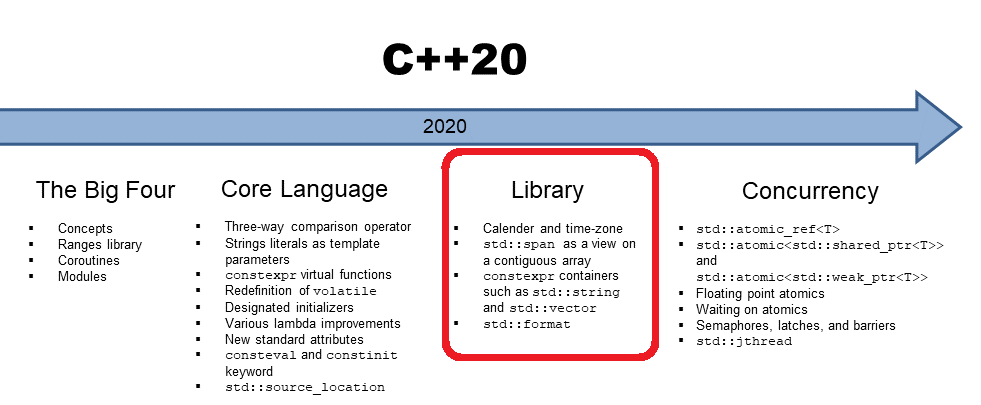
\includegraphics[width=1.2\textwidth, height=1.2\textheight, keepaspectratio]{./imgs/TimelineCpp20_3.png}
	\caption{C++20 Timeline}
	\label{fig:TimelineCpp20_3}
\end{figure}

\subsection{Ranges}

\label{ranges}

%TODO: ranges view

\textsf{\small \textbf{Definizione: } I \textbf{ranges} sono, concettualmente, un paio di iteratori, all'inizio ed alla fine della sequenza ( o una \emph{sentinel} sentinella in certi casi).} \\

\textsf{\small I \textbf{ranges} velocizzano la chiamata alle funzioni della \emph{Libreria degli Algoritmi} in cui al posto di dover passare un iteratore (.begin(), .end()) con i \textbf{ranges} possiamo semplicemente passare l'oggetto, la sequenza stessa.} \break

\subsubsection{Tipi di Ranges}

\textsf{\small I ranges possono essere \emph{input ranges} (possono essere letti), \emph{output ranges} (ci si può scrivere) o entrambi.} \\

\textsf{\small Gli \emph{input ranges}: } \\

\begin{tabular}{|c|c|}
	\hline
	\textbf{Concetto} & \textbf{Descrizione} \\
	\hline
	\textsf{\small \textbf{std::ranges::input\_range}} & \textsf{\small può essere iterato } \\
	\textsf{\small \textbf{}} & \textsf{\small dall'inizio alla fine almeno una volta.} \\
	\hline
	\textsf{\small \textbf{std::ranges::forward\_range}} & \textsf{\small può essere iterato } \\
	\textsf{\small \textbf{}} & \textsf{\small dall'inizio alla fine molteplici volte.} \\
	\hline
	\textsf{\small \textbf{std::ranges::bidirectional\_range}} & \textsf{\small può muoversi all'indietro con \textbf{- -}.} \\
	\hline
	\textsf{\small \textbf{std::ranges::random\_access\_range}} & \textsf{\small si possono saltare gli elementi con \textbf{[]}.} \\
	\hline
	\textsf{\small \textbf{std::ranges::contiguous\_range}} & \textsf{\small gli elementi vengono } \\
	\textsf{\small \textbf{}} & \textsf{\small memorizzati consecutivamente in memoria.} \\
	\hline
\end{tabular}

\textsf{\small Questi concetti sono derivati direttamente dai rispettivi concetti negli iteratori.} \\

\textsf{\small Ci sono anche dei \textbf{ranges} che sono indipendenti dall'\emph{input} o \emph{output}, per esempio \textbf{std::ranges::sized\_range} che richiede che lo spazio di un range sia recuperabile da \textbf{std::ranges::size()}.} \\

\textsf{\small Le \textbf{ranges::views} sono dei \textbf{ranges} che trasformano il \textbf{range} attraverso degli algoritmi o delle operazioni. Le \textbf{views} non possiedono alcuna data eccetto il loro algoritmo e il tempo di costruzione, distruzione o copiatura non dovrebbe dipendere dal numero di elementi che rappresentano.} \\

\textsf{\small I \textbf{ranges} sono definiti nel file di intestazione: \textbf{<ranges>}.} \\

\textsf{\small Di seguito, alcuni esempi degli algoritmi già visti, ma con l'utilizzo dei \textbf{ranges}. } \\

\subsubsection{Operazioni su sequenze non modificabili}

\label{ranges_seq_non_modificabili}

\begin{lstlisting}
	#include <iostream>
	#include <algorithm>
	#include <string_view>
	#include <ranges>
	
	int main()
	{
		// ESEMPIO RANGES::STARTS\_WITH
		std::cout << std::boolalpha << std::ranges::starts_with("luce", "lucertola") << '\n'; //Output: true
		std::cout << std::boolalpha << std::ranges::starts_with("const", "cast") << '\n'; //Output: false
		
		// ESEMPIO RANGES::ENDS\_WITH
		std::cout << std::boolalpha << std::ranges::ends_with("ter", "computer") << '\n'; //Output: true
		std::cout << std::boolalpha << std::ranges::ends_with("asse", "casse") << '\n'; //Output: true
		std::cout << std::boolalpha << std::ranges::ends_with("ada", "scheda") << '\n'; //Output: false
		return 0;
	}
\end{lstlisting}

\subsubsection{Operazioni su sequenze modificabili}

\label{ranges_seq_modificabili}

\begin{lstlisting}
	#include <iostream>
	#include <algorithm>
	#include <vector>
	#include <ranges>
	#include <string>
	#include <random>
	#include <array>
	
	void printContainer(const auto& container)
	{
		for(const auto& o : container)
		{
			std::cout << o << ' ';
		}
		std::cout << '\n';
	}
	
	int main()
	{
		// ESEMPIO RANGES::VIEWS::TRANSFORM
		namespace rn = std::ranges;
		namespace vi = std::ranges::views;
		
		std::vector<int> numbers = { 7, 8, 1, 2, 5, 3 };
		
		auto result = numbers | vi::filter([](int n) {return n % 2 == 0; })
		| vi::transform([](int n) {return n * 2; });
		
		for(const int& n : result)
		{
			std::cout << n << ' ';
		}
	
		//Output: 16 4
		
		// ESEMPIO RANGES::SAMPLE
		constexpr int NUM_OF_LETTERS = 6;
		std::string in = "gjhcioz", out;
		std::sample(in.begin(), in.end(), std::back_inserter(out),
		NUM_OF_LETTERS, std::mt19937{std::random_device{}()});
		std::cout << NUM_OF_LETTERS << " lettere casuali da: " << in << " : " << out << '\n';
		
		//Output: 6 lettere casuali da: gjhcioz : gjcioz
		
		// ESEMPIO RANGES::REPLACE, RANGES::REPLACE\_IF
		std::array<int, 10> arr{5, 7, 4, 2, 8, 6, 1, 9, 0, 3};
		
		std::replace(arr.begin(), arr.end(), 8, 88);
		
		printContainer(arr);
		
		std::replace_if(arr.begin(), arr.end(), 
		std::bind(std::less<int>(), std::placeholders::_1, 3), 33);
		printContainer(arr);
		
		//Output: 5 7 4 2 88 6 1 9 0 3 
		//Output: 5 7 4 33 88 6 33 9 33 3
		return 0;
	}
\end{lstlisting}

\subsubsection{Operazioni su Partizioni}

\label{ranges_partition}

\begin{lstlisting}
	#include <iostream>
	#include <algorithm>
	#include <vector>
	#include <ranges>
	#include <cctype>
	#include <iterator>
	#include <array> // per std::array
	#include <utility> // per std::as\_const
	
	void printContainer(const auto& container)
	{
		for(const auto& o : container)
		{
			std::cout << o << ' ';
		}
		std::cout << '\n';
	}
	
	int main()
	{
		// ESEMPIO RANGES::PARTITION\_COPY
		const auto in = {'N', '0', 'U', 'M', '4', 'B', '9', 'E', '1', '0', 'R', '6'};
		
		std::vector<int> v1(size(in)), v2(size(in));
		
		auto pred = [](char c){ return std::isalpha(c); };
		
		auto result = std::ranges::partition_copy(in, v1.begin(), v2.begin(), pred);
		
		std::ostream_iterator<char> cout {std::cout, " "};
		std::cout << "in = ";
		std::ranges::copy(in, cout);
		std::cout << "\no1 = ";
		std::copy(v1.begin(), result.out1, cout);
		std::cout << "\no2 = ";
		std::copy(v2.begin(), result.out2, cout);
		std::cout << '\n';
		
		//Output: in = N 0 U M 4 B 9 E 1 0 R 6 
		//Output: v1 = N U M B E R 
		//Output: v2 = 0 4 9 1 0 6 
		
		// ESEMPIO RANGES::PARTITION\_POINT
		std::array v = { 1, 2, 3, 4, 5, 6, 7, 8, 9 };
		
		auto is_even = [](int i){ return i % 2 == 0; };
		
		std::ranges::partition(v, is_even);
		
		std::cout << "Dopo la partizione: ";
		printContainer(v);
		
		const auto pp = std::ranges::partition_point(v, is_even);
		const auto i = std::ranges::distance(v.cbegin(), pp);
		std::cout << "Partition point è a: " << i << "; v[" << i << "] = " << *pp << '\n';
		
		std::cout << "Prima partizione (tutti numeri pari): ";
		printContainer(v);
		
		std::cout << "Seconda partizione (tutti numeri dispari): ";
		printContainer(v);
		
		//Output: Dopo la partizione: 8 2 6 4 5 3 7 1 9 
		//Output: Partition point è a: 4; v[4] = 5
		//Output: Prima partizione (tutti numeri pari): 8 2 6 4 5 3 7 1 9 
		//Output: Seconda partizione (tutti numeri dispari): 8 2 6 4 5 3 7 1 9
		
		// ESEMPIO RANGES::IS\_PARTITIONED, RANGES::PARTITION, 
		std::array<int, 9> v;
		
		auto isEven = [](int i){ return i % 2 == 0; };
		auto print = [&](bool o) {
			for (int x : v) std::cout << x << ' ';
			std::cout << (o ? "=> " : "=> non ") << "partizionato\n";
		};
		
		std::iota(v.begin(), v.end(), 1);
		print(std::ranges::is_partitioned(v, isEven));
		
		std::ranges::partition(v, isEven);
		print(std::ranges::is_partitioned(std::as_const(v), isEven));
		
		std::ranges::reverse(v);
		print(std::ranges::is_partitioned(v.cbegin(), v.cend(), isEven));
		print(std::ranges::is_partitioned(v.crbegin(), v.crend(), isEven));
		
		//Output: 1 2 3 4 5 6 7 8 9 => non partizionato
		//Output: 8 2 6 4 5 3 7 1 9 => partizionato
		//Output: 9 1 7 3 5 4 6 2 8 => non partizionato
		//Output: 9 1 7 3 5 4 6 2 8 => partizionato
		
		return 0;
	}
\end{lstlisting}

\subsubsection{Operazioni di Ordinamento}

\label{ranges_sorting}

\begin{lstlisting}
	#include <iostream>
	#include <algorithm>
	#include <vector>
	#include <ranges>
	#include <array>
	
	int main()
	{
		// ESEMPIO RANGES::SORT, RANGES::IS\_SORTED
		namespace ranges = std::ranges;
		
		std::array arr {7, 8, 4, 2, 5, 3};
		
		ranges::copy(arr, std::ostream_iterator<int>(std::cout, " "));
		std::cout << ": is_sorted: " << std::boolalpha
		<< ranges::is_sorted(arr) << '\n';
		
		ranges::sort(arr);
		
		ranges::copy(arr, std::ostream_iterator<int>(std::cout, " "));
		std::cout << ": is_sorted: "
		<< ranges::is_sorted(ranges::begin(arr), 
		ranges::end(arr)) << '\n';
		return 0;
	}
\end{lstlisting}

\subsubsection{Operazioni su ricerca binaria}

\label{ranges_binary_search}

\begin{lstlisting}
	#include <iostream>
	#include <algorithm>
	#include <vector>
	#include <ranges>
	
	int main()
	{
		namespace ranges = std::ranges;
		
		// ESEMPIO RANGES::LOWER\_BOUND, RANGES::UPPER\_BOUND
		std::vector<int> vec = { 4, 1, 7, 3, 2, 3, 3, 8, 4, 4, 5, 8, 6 };
		
		{
			auto lower = ranges::lower_bound(vec.begin(), vec.end(), 4);
			auto upper = ranges::upper_bound(vec.begin(), vec.end(), 4);
			
			ranges::copy(lower, upper, std::ostream_iterator<int>(std::cout, " "));
			std::cout << '\n'; //Output: 8 4 4
			
		}
		{
			auto lower = ranges::lower_bound(vec, 3);
			auto upper = ranges::upper_bound(vec, 3);
			
			ranges::copy(lower, upper, std::ostream_iterator<int>(std::cout, " "));
			std::cout << '\n'; //Output: 7 3 2 3 3
		}
	
		// ESEMPIO RANGES::BINARY\_SEARCH
		constexpr static auto haystack = {1, 3, 4, 8, 9, 5};
		constexpr static auto needles = {1, 2, 3};
		
		for (const int needle : needles) {
			std::cout << "Cercando il: " << needle << ": ";
			std::ranges::binary_search(haystack, needle) ? std::cout << "trovato\n" : std::cout << "non trovato!\n";
		}
	
		//Output: Cercando il: 1: trovato
		//Output: Cercando il: 2: non trovato!
		//Output: Cercando il: 3: trovato
		return 0;
	}
\end{lstlisting}

\subsubsection{Operazioni di Fusione | Merge}

\label{ranges_merge}

\begin{lstlisting}
	#include <iostream>
	#include <algorithm>
	#include <vector>
	#include <ranges>
	
	void printContainer(const auto& container)
	{
		for(const auto& o : container)
		{
			std::cout << o << ' ';
		}
		std::cout << '\n';
	}
	
	int main()
	{
		// ESEMPIO RANGES::MERGE
		std::vector<int> in1, in2, out;
		
		in1 = {1, 2, 3, 4, 5};
		in2 = {      3, 4, 5, 6, 7};
		out.resize(in1.size() + in2.size());
		const auto ret = std::ranges::merge(in1, in2, out.begin());
		
		printContainer(in1);
		std::cout << "+ " << '\n';
		printContainer(in2);
		std::cout << "= " << '\n';
		printContainer(out);
		
		//Output: 1 2 3 4 5 
		//Output: + 
		//Output: 3 4 5 6 7 
		//Output: = 
		//Output: 1 2 3 3 4 4 5 5 6 7
		return 0;
	}
\end{lstlisting}

\subsubsection{Operazioni sugli Insiemi}

\label{ranges_set}

\begin{lstlisting}
	#include <iostream>
	#include <algorithm>
	#include <vector>
	#include <ranges>
	
	void printContainer(const auto& container)
	{
		for(const auto& o : container)
		{
			std::cout << o << ' ';
		}
		std::cout << '\n';
	}
	
	int main()
	{
		// ESEMPIO RANGES::SET\_INTERSECTION
		std::vector<int> v1 = {8, 2, 7, 9, 4, 5, 6 };
		std::vector<int> v2 = {2, 3, 4, 3, 5, 7};
		std::vector<int> v3;
		
		std::ranges::sort(v1.begin(), v1.end());
		std::ranges::sort(v2.begin(), v2.end());
		
		std::ranges::set_intersection(v1, v2, std::back_inserter(v3));
		
		std::cout << "v1 contiene: ";
		printContainer(v1); 
		
		//Output: v1 contiene: 2 4 5 6 7 8 9 
		
		std::cout << "v2 contiene: ";
		printContainer(v2); 
		
		//Output: v2 contiene: 2 3 3 4 5 7 
		
		std::cout << "l'intersezione v3 contiene: ";
		printContainer(v3);
		
		//Output: l'intersezione v3 contiene: 2 4 5 7
		
		// ESEMPIO RANGES::SET\_SYMMETRIC\_DIFFERENCE
		const auto in1 = {1, 3, 4,    6, 7, 9};
		const auto in2 = {1,    4, 5, 6,    9};
		
		std::vector<int> out;
		
		std::ranges::set_symmetric_difference(in1, in2, std::back_inserter(out));
		
		std::cout << "in1 contiene: ";
		printContainer(in1);
		
		//Output: in1 contiene: 1 3 4 6 7 9
		
		std::cout << "in2 contiene: ";
		printContainer(in2);
		
		//Output: in2 contiene: 1 4 5 6 9
		
		std::cout << "la differenza simmetrica out contiene: ";
		printContainer(out);
		
		//Output: la differenza simmetrica out contiene: 3 5 7 
		
		// ESEMPIO RANGES::SET\_UNION
		std::vector<int> vec1, vec2, vec3;
		
		vec1 = {1, 2, 3, 4, 5};
		vec2 = {      3, 4, 5, 6, 7};
		vec3.resize(vec1.size() + vec2.size());
		std::ranges::set_union(vec1, vec2, vec3.begin());
		
		std::cout << "vec1 contiene: ";
		printContainer(vec1);
		
		//Output: vec1 contiene: 1 2 3 4 5 
		
		std::cout << "vec2 contiene: ";
		printContainer(vec2);
		
		//Output: vec2 contiene: 3 4 5 6 7
		
		std::cout << "vec3 contiene: ";
		printContainer(vec3);
		
		//Output: vec3 contiene: 1 2 3 4 5 6 7 0 0 0 
		
		return 0;
	}
\end{lstlisting}

\subsubsection{Operazioni su Heap}

\label{ranges_heap}

\begin{lstlisting}
	#include <iostream>
	#include <algorithm>
	#include <vector>
	#include <ranges>
	#include <array>
	
	void printContainer(const auto& container)
	{
		for(const auto& o : container)
		{
			std::cout << o << ' ';
		}
		std::cout << '\n';
	}
	
	int main()
	{
		// ESEMPIO RANGES::MAKE\_HEAP, RANGES::POP\_HEAP
		std::array v { 4, 7, 5, 1, 3, 9, 8, 6, 5, 2 };
		std::cout << "Inizialmente: ";
		printContainer(v);
		
		//Output: Inizialmente: 4 7 5 1 3 9 8 6 5 2
		
		std::ranges::make_heap(v);
		std::cout << "make_heap: ";
		printContainer(v);
		
		//Output: make\_heap: 9 7 8 6 3 5 4 1 5 2
		
		print("converto l'heap in un array ordinato:");
		for (auto n {std::ssize(v)}; n >= 0; --n) {
			std::ranges::pop_heap(v.begin(), v.begin() + n);
			print("[ ", v.cbegin(), v.cbegin() + n, "]  ");
			print("[ ", v.cbegin() + n, v.cend(), "]\n");
		}
		
		//Output:
		[ 8 7 5 6 3 2 4 1 5 9 ]  [ ]
		[ 7 6 5 5 3 2 4 1 8 ]  [ 9 ]
		[ 6 5 5 1 3 2 4 7 ]  [ 8 9 ]
		[ 5 5 4 1 3 2 6 ]  [ 7 8 9 ]
		[ 5 3 4 1 2 5 ]  [ 6 7 8 9 ]
		[ 4 3 2 1 5 ]  [ 5 6 7 8 9 ]
		[ 3 1 2 4 ]  [ 5 5 6 7 8 9 ]
		[ 2 1 3 ]  [ 4 5 5 6 7 8 9 ]
		[ 1 2 ]  [ 3 4 5 5 6 7 8 9 ]
		[ 1 ]  [ 2 3 4 5 5 6 7 8 9 ]
		[ ]  [ 1 2 3 4 5 5 6 7 8 9 ]
		
		// ESEMPIO RANGES::SORT\_HEAP
		std::array v {4, 9, 4, 7, 6, 12};
		std::cout << "array originale: ";
		printContainer(v);
		
		//Output: array originale: 4 9 4 7 6 12
		
		std::ranges::make_heap(v);
		std::cout << "dopo il make_heap: ";
		printContainer(v);
		
		//Output: dopo il make\_heap: 12 9 4 7 6 4 
		
		std::ranges::sort_heap(v);
		std::cout << "dopo il sort_heap: ";
		printContainer(v);
		
		//Output: dopo il sort\_heap: 4 4 6 7 9 12
		return 0;
	}
\end{lstlisting}

\subsubsection{Operazioni su Min/Max}

\label{ranges_minmax}

\begin{lstlisting}
	#include <iostream>
	#include <algorithm>
	#include <vector>
	#include <ranges>
	
	int main()
	{
		// ESEMPIO RANGES::MIN\_ELEMENT, RANGES::MAX\_ELEMENT
		std::vector<int> v{ 2, 6, -17, 2, 1, 9 };
		
		namespace ranges = std::ranges;
		
		auto result = ranges::max_element(v.begin(), v.end());
		std::cout << "elemento massimo a: " << ranges::distance(v.begin(), result) << '\n'; //Output: elemento massimo a: 5
		
		auto absCompare = [](int a, int b) { return (std::abs(a) < std::abs(b)); };
		result = ranges::max_element(v, absCompare);
		std::cout << "elemento massimo (assoluto) a: " << ranges::distance(v.begin(), result) << '\n'; //Output: elemento massimo (assoluto) a: 2
		
		auto result2 = ranges::min_element(v.begin(), v.end());
		std::cout << "elemento minimo a: " << ranges::distance(v.begin(), result) << '\n'; //Output: elemento minimo a: 2
		
		result = ranges::min_element(v, absCompare);
		std::cout << "elemento minimo (assoluto) a: " << ranges::distance(v.begin(), result2) << '\n'; //Output: elemento minimo (assoluto) a: 2
		
		// ESEMPIO RANGES::MINMAX
		const auto v = { 5, 1, 3, 4, 2, 7, 5, 9 };
		const auto [min, max] = ranges::minmax_element(v);
		std::cout << "minimo: " << *min << ", all'indice: [" << ranges::distance(v.begin(), min) << "]\n" 
		<< "massimo: " << *max << ", all'indice: [" << ranges::distance(v.begin(), max) << "]\n";
		
		//Output: minimo: 1, all'indice: [1]
		//Output: massimo: 9, all'indice: [7]
		
		return 0;
	}
\end{lstlisting}

\subsubsection{Operazioni di Comparazione}

\label{ranges_compare}

\begin{lstlisting}
	#include <iostream>
	#include <algorithm>
	#include <vector>
	#include <ranges>
	#include <string_view>
	
	// Palindromo: sequenza di caratteri che letta al contrario rimane invariata.
	constexpr bool isPalindrome(const std::string_view s)
	{
		namespace views = std::views;
		auto forward = s | views::take(s.size() / 2);
		auto backward = s | views::reverse | views::take(s.size() / 2);
		return std::ranges::equal(forward, backward);
	}
	
	void test(const std::string_view s)
	{
		std::cout << s << (isPalindrome(s) ? " è" : " non è") << " un palindromo\n";
	}
	
	int main()
	{
		// ESEMPIO RANGES::EQUAL
		test("radar"); //Output: radar è un palindromo
		test("ciao"); //Output: ciao non è un palindromo
		return 0;
	}
\end{lstlisting}

\subsubsection{Operazioni su Permutazioni}

\label{ranges_permutation}

\begin{lstlisting}
	#include <iostream>
	#include <algorithm>
	#include <vector>
	#include <ranges>
	
	auto& operator<< (auto& os, std::ranges::forward_range auto const& v) {
		os << "{ ";
			for (auto const& e : v) os << e << ' ';
			return os << "}";
	}
	
	int main()
	{
		// ESEMPIO RANGES::IS\_PERMUTATION
		static constexpr auto r1 = {1,2,3,4,5};
		static constexpr auto r2 = {3,5,4,1,2};
		static constexpr auto r3 = {3,5,4,1,1};
		
		static_assert(
		std::ranges::is_permutation(r1, r1) &&
		std::ranges::is_permutation(r1, r2) &&
		std::ranges::is_permutation(r2, r1) &&
		std::ranges::is_permutation(r1.begin(), r1.end(), r2.begin(), r2.end())
		);
		
		std::cout << std::boolalpha << "is_permutation( " << r1 << ", " << r2 << " ): " << std::ranges::is_permutation(r1, r2) << '\n' << "is_permutation( " 
		<< r1 << ", " << r3 << " ): " << std::ranges::is_permutation(r1, r3) << '\n';
		
		//Output: is\_permutation( { 1 2 3 4 5 }, { 3 5 4 1 2 } ): true
		//Output: is\_permutation( { 1 2 3 4 5 }, { 3 5 4 1 1 } ): false
		return 0;
	}
\end{lstlisting}

\subsubsection{Operazioni numeriche}

\label{ranges_numeric}

\begin{lstlisting}
	#include <iostream>
	#include <algorithm>
	#include <vector>
	#include <ranges>
	#include <numeric>
	#include <list>
	#include <random>
	
	int main()
	{
		// ESEMPIO RANGES::IOTA
		std::list<int> l(10);
		std::ranges::iota(l.begin(), l.end(), -4);
		
		std::vector<std::list<int>::iterator> v(l.size());
		std::ranges::iota(v, l.begin());
		
		std::ranges::shuffle(v, std::mt19937{std::random_device{}()});
		
		std::cout << "Contenuti della lista: ";
		for(auto n: l) std::cout << n << ' ';
		std::cout << '\n';
		
		//Output: Contenuti della lista: -4 -3 -2 -1 0 1 2 3 4 5
		
		std::cout << "Contenuti della lista, mischiati: ";
		for(auto i: v) std::cout << *i << ' ';
		std::cout << '\n';
		
		//Output: Contenuti della lista, mischiati: 0 -1 3 4 -4 1 -2 -3 2 5
		
		return 0;
	}
\end{lstlisting}

\subsubsection{Operazioni su memoria non inizializzata}

\label{ranges_uninitialized_memory}

\begin{lstlisting}
	#include <iostream>
	#include <algorithm>
	#include <vector>
	#include <ranges>
	#include <memory>
	#include <string>
	
	int main()
	{
		// ESEMPIO RANGES::UNINITIALIZED\_FILL\_N, RANGES::DESTROY
		constexpr int n {3};
		alignas(alignof(std::string)) char out[n * sizeof(std::string)];
		
		try
		{
			auto first {reinterpret_cast<std::string*>(out)};
			auto last = std::ranges::uninitialized_fill_n(first, n, "C++");
			
			for (auto it {first}; it != last; ++it) {
				std::cout << *it << '\n';
			}
			
			std::ranges::destroy(first, last);
		}
		catch(...)
		{
			std::cout << "Exception!\n";
		}
		
		//Output: C++
		//Output: C++
		//Output: C++
		return 0;
	}
\end{lstlisting}

\subsubsection{Tipi di Ritorno}

%TODO: aggiungere spiegazione su questi (fare dei commenti).
\begin{lstlisting}
	#include <iostream>
	#include <algorithm>
	#include <vector>
	#include <ranges>
	
	int main()
	{
		// ESEMPIO RANGES::IN\_FUN\_RESULT
		int v[] { 1, 2, 3 };
		
		const auto [last, negate] = std::ranges::for_each_n(v, std::size(v),
		[](int& x) { return x = -x; });
		
		const auto result = std::ranges::for_each(std::cbegin(v), last,
		[](int x) { std::cout << x << ' '; });
		std::cout << "| ";
		
		std::ranges::for_each(v, negate);
		std::ranges::for_each(v, result.fun);
		std::cout << '\n';
		
		//Output: -1 -2 -3 | 1 2 3
		
		// ESEMPIO RANGES::MIN\_MAX\_RESULT
		constexpr static auto v2 = {3, 1, 4, 1, 5, 9, 2};
		{
			constexpr auto result2 = std::ranges::minmax(v2);
			static_assert(1 == result2.min && 9 == result2.max);
		}
		{
			constexpr auto result2 = std::ranges::minmax_element(v2);
			static_assert(1 == *result2.min && 9 == *result2.max);
		}
		
		//Output: [nessun output, non stiamo stampando niente]
		
		// ESEMPIO RANGES::IN\_FOUND\_RESULT
		int v3[] { 1, 2, 3 };
		
		const auto result3 = std::ranges::next_permutation(v3);
		
		std::ranges::for_each(std::cbegin(v3), result3.in, [](int e){std::cout << e << ' ';});
		
		std::cout << std::boolalpha << "\n" "result3.found: " << result3.found << '\n';
		
		//Output: 1 3 2 
		//Output: result3.found: true
		return 0;
	}
\end{lstlisting}

\newpage

\subsection{Concepts}

\label{concepts}

\textsf{\small \textbf{Definizione: } I \textbf{Concepts} sono un nuovo approccio rivoluzionario del \textbf{C++20} per trattare i \textbf{templates}. Permettono di porre dei vincoli (\emph{constraints}) ai parametri dei \textbf{template} per migliorare la leggibilità del codice, la velocità al momento della compilazione e fornire dei migliori messaggi d'errore.} \\

\textsf{\small Il \textbf{C++20} fornisce due nuove keywords: \textbf{concept} e \textbf{requires} ed un insieme di \textbf{concepts} predefiniti dalla \emph{Libreria Standard}.} \\

\textsf{\small Per poter usufruire di queste funzionalità sarà necessario includere \textbf{<concepts>}.} \\

\subsubsection{concept}

\begin{lstlisting}
	#include <iostream>
	#include <concepts>
	#include <type_traits>
	#include <string>
	
	// template<typename T>
	// concept conceptName = conceptExpression;
	
	template<class T>
	concept integral = std::is_integral_v<T>; // std::is\_integral\_v da <type\_traits> restituisce true o false se il parametro passato è di tipo intero.
	
	template<integral T> // Questo al posto del tipico typename T
	class MyClass {
		public:
			MyClass(T x)
			{
				this->x = x;   
			}
		
		private:
			T x;
	};

	template<typename T>
	class MyClass2 {
		public:
			MyClass(T x)
			{
				this->x = x;   
			}
		
		private:
			T x;
	};

	int main()
	{
		std::string s = "ciao";
		
		int x = 5;
		
		MyClass<int> instance(s); //Errore template argument deduction/substitution failed. (passiamo una stringa, quando invece c'è il vincolo che i parametri T siano interi)
		
		MyClass<double> instance2(7.12); //Errore requires integral<T> (il tipo della classe è double quando noi invece vogliamo un tipo intero)
		
		MyClass instance3(x); // Questo va bene. (soddisfa il vincolo che sia intero)
		
		MyClass<int> instance4(x); // Questo va bene. (soddisfa il vincolo che sia intero)
		
		MyClass2<double> myClass2Instance(5.55); // Non da errore perché stiamo usando la classe senza il vincolo.
		
		MyClass2 myClass2Instance2(s); // Non da errore perché stiamo usando la classe senza il vincolo.
		
		return 0;
	}
\end{lstlisting}

\textsf{\small In questo esempio, abbiamo usato la keyword \textbf{concept} per definire una classe template con un vincolo, in questo caso il vincolo che la classe sia di tipo integrale, ovvero sia un numero intero e quindi non andavano bene nè le istanze double nè string nè qualsiasi altri tipo diverso dagli interi.} \\

\begin{lstlisting}
	#include <iostream>
	#include <concepts>
	
	template<typename T>
	concept hasStringDataMember = requires(T v) { 
		{ v.name } -> std::convertible_to<std::string>; 
	};
	
	class Person {
		public:
		int age { 0 };
		std::string name;
	};
	
	class Box {
		public:
		double weight { 0.0 };
		double volume { 0.0 };
	};
	
	int main()
	{
		static_assert(hasStringDataMember<Person>);
		static_assert(!hasStringDataMember<Box>); // Qui non da errore perché abbiamo messo ! altrimenti lo darebbe perché Box non ha un membro di tipo std::string chiamato name.
		return 0;
	}
\end{lstlisting}

\subsubsection{requires}

\begin{lstlisting}
	#include <iostream>
	#include <concepts>
	#include <string>
	#include <numeric> // per std::accumulate
	#include <type_traits>
	
	// ESEMPIO REQUIRES 1
	template <typename T>
	requires std::convertible_to<T, std::string>
	void func(const T& x) {
		std::string s = x;
	}

	// ESEMPIO REQUIRES 2
	template<typename T>
	requires std::integral<T> || std::floating_point<T> // o numeri interi o con la virgola (std::integral e std::floating\_point vengono dal'header <concepts>)
	constexpr double average(const std::vector<T> &vec) {
		const double sum = std::accumulate(vec.cbegin(), vec.cend(), (T)0);        
		return sum / vec.size();
	}

	int main()
	{
		// ESEMPIO REQUIRES 1
		const std::string s = "ciao";
		const int x = 7;
		
		func(x); //Errore: perché x è di tipo intero e invece noi abbiamo bisogno di un tipo convertibile a std::string.
		
		func(s); // Questo va bene.
		
		// ESEMPIO REQUIRES 2
		std::vector<int> v = { 7, 8, 12, 5};
		
		std::cout << average(v) << std::endl; //Output: 8 (funziona perché è intero)
		
		std::vector<float> v2 = { 5.7, 12.4, 8.8, 9.1 };
		
		std::cout << average(v2) << std::endl; //Output: 9 (funziona perché è un numero con la virgola) (funziona anche il double, non solo il float)
		
		std::vector<bool> v3 = { true, false, true, true, false };
		
		std::cout << average(v3) << std::endl; //Output: 0.2 (funziona perché i booleani sono dei numeri, ovvero true = 1; false = 0)
		
		std::vector<std::string> v4 = { "ciao", "a", "tutti" };
		
		std::cout << average(v4) << std::endl; //Output: Errore constraints not satisfied (vincoli non soddisfatti perché non è nè un intero nè un numero con la virgola)
		return 0;
	}
\end{lstlisting}

\textsf{\small In questo esempio abbiamo visto come \textbf{requires} ci permette di validare che un data variabile sia dia una determinata tipologia.} \\

\begin{lstlisting}
	#include <iostream>
	#include <concepts>
	
	// ESEMPIO REQUIRES 1
	template <typename T>
	concept addable = requires (T a, T b) {
		a+b;
	};
	
	void function(addable auto x) {
		std::cout << x << " è sommabile!" << std::endl;    
	}

	// ESEMPIO REQUIRES 2
	template <typename T>
	requires std::integral<T> ||
	(std::invocable<T> &&
	std::integral<typename std::invoke_result<T>::type>)
	void function2(const T& x) {
		if constexpr (std::invocable<T>) {
			std::cout << "Il risultato della chiamata è: " << x() << "\n";
		} else {
			std::cout << "Il valore è: " << x << "\n";
		}
	}
	
	int main()
	{
		// ESEMPIO REQUIRES 1
		function(3); //Output: 3 è sommabile!
		
		function("Hello World!"); //Output: Errore
		
		// ESEMPIO REQUIRES 2
		function2(6); //Output: Il valore è: 6 (va bene perché è un intero, quindi va nell'else)
		function2( []() { return 3; } ); //Output: (va bene perché è invocabile, restituisce un intero, va nell'if)
		
		function2(3.3); //Output: Errore perchè non è un intero nè un invocabile
		function2( []() { return 3.3; } ); //Output: Errore perchè è un invocabile, ma restituisce un valore non intero.
		return 0;
	}
\end{lstlisting}

\textsf{\small La \emph{Libreria Standard} fornisce vari \textbf{concepts} predefiniti nell'header \textbf{<concepts>}, come quelli visti \textbf{std::integral} e \textbf{std::floating\_point} e tanti altri.} \\

%TODO: volendo potrei elencarli, però senza spiegarli è un po' inutile.

\subsubsection{Concepts fixano, sposano e rimpiazzano SFINAE}

\textsf{\small \textbf{SFINAE} (\emph{Substitution Failure Is Not An Error}), concetto trattato nel capitolo \emph{Concetti Avanzati} a pag.\textbf{\pageref{SFINAE}} viene praticamente sostituito dai \textbf{Concepts} che possono fare la stessa cosa, ma molto meglio.} \\

\newpage

\subsection{Modules}

\textsf{\small \textbf{Definizione: } I \textbf{Modules} permettono di velocizzare un programma attraverso l'importazione di \textbf{moduli}, porzioni di codice, invece di \textbf{includere} un \textbf{header}.} \\

\textsf{\small Quindi, in un certo senso i \textbf{modules} servono in parte, ma non del tutto sostituire gli \textbf{headers}.} \\

\textsf{\small I \textbf{Modules} forniscono due nuove keywords: \textbf{export} e \textbf{import}.} \break

\textsf{\small Negli \textbf{headers} il \emph{preprocessore} essenzialmente copierà ed incollerà i contenuti dell'\textbf{header} al posto dell'\textbf{include} e questo per ogni file di implementazione nel programma.} \\

\textsf{\small I \textbf{Modules} sono come gli \textbf{headers}, ma sono anche una \textbf{unità di traduzione} (\emph{translation unit}), proprio per questo viene compilata separatamente e solo una volta. La keyword \textbf{import} ci permette di ottenere accesso alle dichiarazioni della libreria. } \\

\textsf{\small Il vantaggio principale è che i \textbf{modules} vengono \emph{parsati} a livello di \textbf{abstract syntax tree} (\emph{ABT}) dal compilatore.} \\

\textsf{\small Questo ci permette una serie di vantaggi: } \\

\begin{enumerate}
	\item \textsf{\small \textbf{Isolamento} : perché un'unità di modulo è una unità di traduzione separata: possiede la sua serie di macros, dichiarazioni, direttive che non influenzano chi lo \emph{importa}.}
	\item \textsf{\small \textbf{Controllo dell'Interfaccia} : perché può dichiarare entità con un link interno, con l'\textbf{export}.}
	\item \textsf{\small \textbf{Deduplicazione} : perché in molti casi non sarà più necessario fornire una dichiarazione in un header file.}
	\item \textsf{\small \textbf{One Definition Rule violation avoidance} (\emph{ODR}) : un modulo può definire un'entità solo una volta e fornire quella definizione ai clienti.}
	\item \textsf{\small \textbf{Ordine di inizializzazione delle variabili non-locali} : perché l'\textbf{import} stabilisce un ordine di dipendenza tra le \emph{unità di traduzione} che contengono (uniche) definizioni di variabili.}
	\item \textsf{\small \textbf{Dichiarazioni di moduli privati} : le entità dichiarate in un modulo che non sono esportate e non hanno un link interno sono usabili dalle \emph{unità di traduzione} stesse nel modulo.}
	\item \textsf{\small \textbf{Stabilità ABI} : le regole dell'\textbf{inline} sono state aggiustate per supportare una strategia d'implementazione dove le funzioni \emph{non-inline} possono servire come frontiera \emph{ABI} per gli aggiornamenti delle librerie condivise.}
	\item \textsf{\small \textbf{Velocità di compilazione} : perché i contenuti dei moduli non devono essere \emph{riparsati}, in molti casi questo velocizza i tempi di compilazione.}
	%\item \textsf{\small \textbf{Strumentazione} : }
\end{enumerate}

\begin{lstlisting}
	// Mathematics.cpp
	export module Mathematics;
	export auto plus(auto x, auto y) -> decltype(x+y) {
		return x + y;
	}
	export namespace Mathematics {
		auto minus(auto x, auto y) -> decltype(x-y) {
			return x - y;  
		}   
	}
	void this_function_will_not_be_exported() {}
	
	// In un altro file: main.cpp
	import <iostream>;
	import Mathematics;
	int main() {
		std::cout << "1+2 = " <<  plus(1,2) << "\n"; //Output: 3
		std::cout << "3-2 = " << Mathematics::minus(3,2) 
		<< "\n"; //Output: 1
		return 0;
	}
\end{lstlisting}

\textsf{\small Abbiamo importato il modulo \emph{Mathematics} e abbiamo usufruito delle sue funzioni nel file \emph{main.cpp}. La funzione \emph{plus} l'abbiamo chiamata direttamente, mentre la \emph{minus} l'abbiamo chiamata con \emph{Mathematics::} visto che si trovava all'interno del \emph{namespace}.} \\

\begin{lstlisting}
	export module helloworld;
	
	export const char* getHelloWorld()
	{
		return "Hello World!";
	}

	// In un altro file: main.cpp
	#import helloworld;
	
	#include <iostream>
	
	int main()
	{
		std::cout << getHelloWorld() << std::endl; //Output: Hello World!
		return 0;
	}
\end{lstlisting}

\textsf{\small In questo esempio, abbiamo il nostro modulo \emph{helloworld} con una singola funzione che restituisce un \emph{const char*} e lo abbiamo importato in un file con la keyword \textbf{import} ed abbiamo usato la funzione al suo interno.} \\

\subsubsection{Modules Partitions}

\textsf{\small Le \textbf{modules partitions} servono per suddividere in più file un \textbf{module}. Le partizioni sono accessibili solo dal modulo principale, devono essere una singola unità (un singolo file), ma possono essere delle unità di interfaccia (gli \emph{export}) o una solo un'unità. Ma se l'unità è un'unità di interfaccia allora deve essere riesportata nel modulo principale \emph{export import :partition;}. Il modulo principale avrà accesso a tutte le partizioni, anche se non sono segnate come \emph{export}.} \\

\begin{lstlisting}
	// helloworld.cpp
	export module helloworld;
	
	export import :english;
	export import :spanish;
	export import :italian;
	
	// helloworld\_english.cpp
	export module helloworld:english;
	
	export const char* getHelloWorldEng()
	{
		return "Hello World!";
	}

	// helloworld\_spanish.cpp
	export module helloworld:spanish;
	
	export const char* getHelloWorldEs()
	{
		return "¡Hola Mundo!";
	}

	// helloworld\_italian.cpp
	export module helloworld:italian;

	export const char* getHelloWorldIta()
	{
		return "Ciao Mondo!";
	}

	// In un altro file: main.cpp
	import helloworld;
	
	#include <iostream>
	#include <cstdlib>
	
	int main()
	{
		int scelta;
		std::cout << "0. Inglese" << '\n';
		std::cout << "1. Spagnolo" << '\n';
		std::cout << "2. Italiano" << '\n';
		std::cout << "Scelta: ";
		std::cin >> scelta;
		
		switch(scelta)
		{
			case 1:
				std::cout << getHelloWorldEs() << std::endl;
				break;
			case 2:
				std::cout << getHelloWorldIta() << std::endl;
				break;
			case 0:
			default:
				std::cout << getHelloWorldEng() << std::endl;
				break;
		}
		return 0;
	}
\end{lstlisting}

\textsf{\small Qui abbiamo creato un modulo chiamato \emph{helloworld} con tre partizioni: \emph{english}, \emph{spanish}, \emph{italian}. } \\ 

\textsf{\small La sintassi \emph{export module <nome-modulo>:<nome-partizione>} dichiara che il dato modulo è una partizione d'interfaccia appartenente a \emph{<nome-modulo>} con la partizione chiamata \emph{<nome-partizione>}.} \\

\textsf{\small La sintassi \emph{import :<nome-partizione>} importa la partizione chiamata \emph{<nome-partizione>}.} \\

\textsf{\small La sintassi \emph{export import :<nome-partizione>} rende l'entità esportata nel modulo partizione visibile come parte del modulo interfaccia.} \\

\subsubsection{Module Implementation}

\textsf{\small È un modulo che non ha la keyword \emph{export} prima della keyword \emph{module} nel suo modulo.} \\

\textsf{\small Le entità dichiarate in una unità d'implementazione sono visibili solo nel modulo in cui fanno parte.} \\

\begin{lstlisting}
	// helloworld.cpp
	export module helloworld;
	
	import :english;
	import :spanish;
	import :italian;
	
	export const char* getHelloWorldEng();
	export const char* getHelloWorldEs();
	export const char* getHelloWorldIta();
	
	// helloworld\_english.cpp
	module helloworld:english;
	
	const char* getHelloWorldEng() 
	{
		return "Hello world!";
	}

	// helloworld\_spanish.cpp
	module helloworld:spanish;
	
	const char* getHelloWorldEs() 
	{
		return "¡Hola Mundo!";
	}

	// helloworld\_italian.cpp
	module helloworld:italian;
	
	const char* getHelloWorldIta() 
	{
		return "Ciao Mondo";
	}
\end{lstlisting}

\textsf{\small Questo era il nostro precedente esempio se usiamo le \emph{unità d'implementazione}.} \\

\textsf{\small Abbiamo visto qui solo uno spunto dell'importanza e della potenza dei \textbf{Modules}, ma è possibile approfondire molto di più l'argomento.} \\

\newpage

\subsection{Coroutines}

\textsf{\small \textbf{Definizione: } Le \textbf{coroutines} sono delle funzioni che sospendono l'esecuzione per poi riprenderla più tardi.} \\

\textsf{\small Sono una struttura generale di controllo dove il flusso di controllo è passato tra due differenti routine senza ritorno.} \\

\begin{figure}[H]
	\centering
	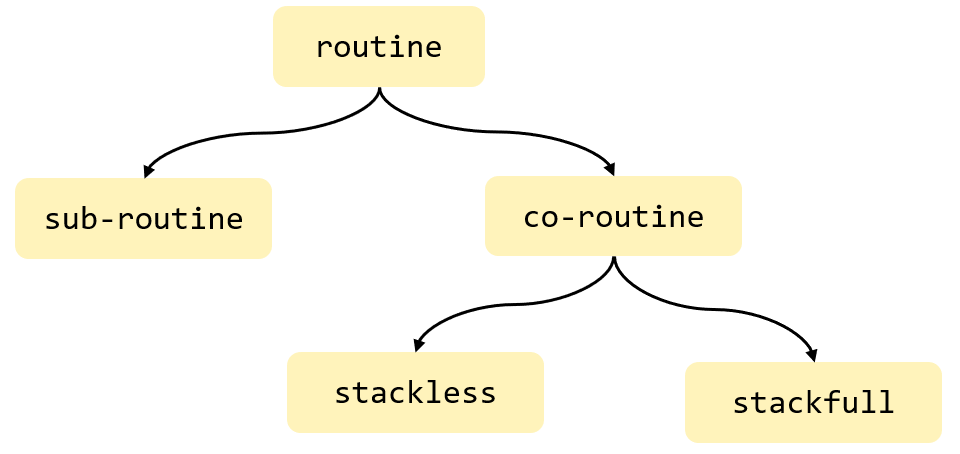
\includegraphics[width=1\textwidth, height=1\textheight, keepaspectratio]{./imgs/C++20-Coroutine-Under-The-Hood.png}
	\caption{C++20 Coroutines in general}
	\label{fig:coroutines_in_general}
\end{figure}

\begin{itemize}
	\item \textsf{\small Una \textbf{coroutine} è una funzione che: }
	\begin{enumerate}
		\item \textsf{\small Contiene le keywords: \textbf{co\_await}, \textbf{co\_yield} e/o \textbf{co\_return}.}
		\item \textsf{\small Usano un tipo di ritorno per specificare una \emph{promessa}.}
	\end{enumerate}
	\item \textsf{\small Più in generale, le \textbf{coroutine} del \textbf{C++20} consistono in:}
	\begin{itemize}
		\item \textsf{\small Promise (Promessa)}
		\begin{itemize}
			\item \textsf{\small Definisce il comportamento della coroutine nel complesso.}
			\item \textsf{\small Agisce come comunicatore tra il chiamante e la coroutine chiamata.}
		\end{itemize}
		\item \textsf{\small Awaiter}
		\begin{itemize}
			\item \textsf{\small Controlla il comportamento di sospensione e di ripresa.}
		\end{itemize}
		\item \textsf{\small Coroutine Handle}
		\begin{itemize}
			\item \textsf{\small Controlla il comportamento di esecuzione.}
		\end{itemize}
	\end{itemize}
\end{itemize}

\subsubsection{A cosa servono le coroutines?}

\textsf{\small  Le \textbf{coroutines} forniscono un alto livello di \emph{concorrenza} con molto poco \emph{overhead}.} \\

\textsf{\small Una \textbf{coroutine} si può sospendere in un predeterminato punto, quindi si può evitare di \emph{lockare} (bloccare) le strutture dati condivise.} \\

\textsf{\small Con i \emph{threads} ogni \emph{thread} necessita di un proprio stack, quindi l'utilizzo di memoria cresce linearmente, mentre con le \textbf{coroutines}, il numero di esse che si ha non ha una diretta relazione con l'utilizzo di memoria. Per la maggior parte dei casi, i \textbf{coroutines} sono una scelta ottimale visto che son più veloci rispetto ai \emph{threads}. } \\

\begin{figure}[H]
	\centering
	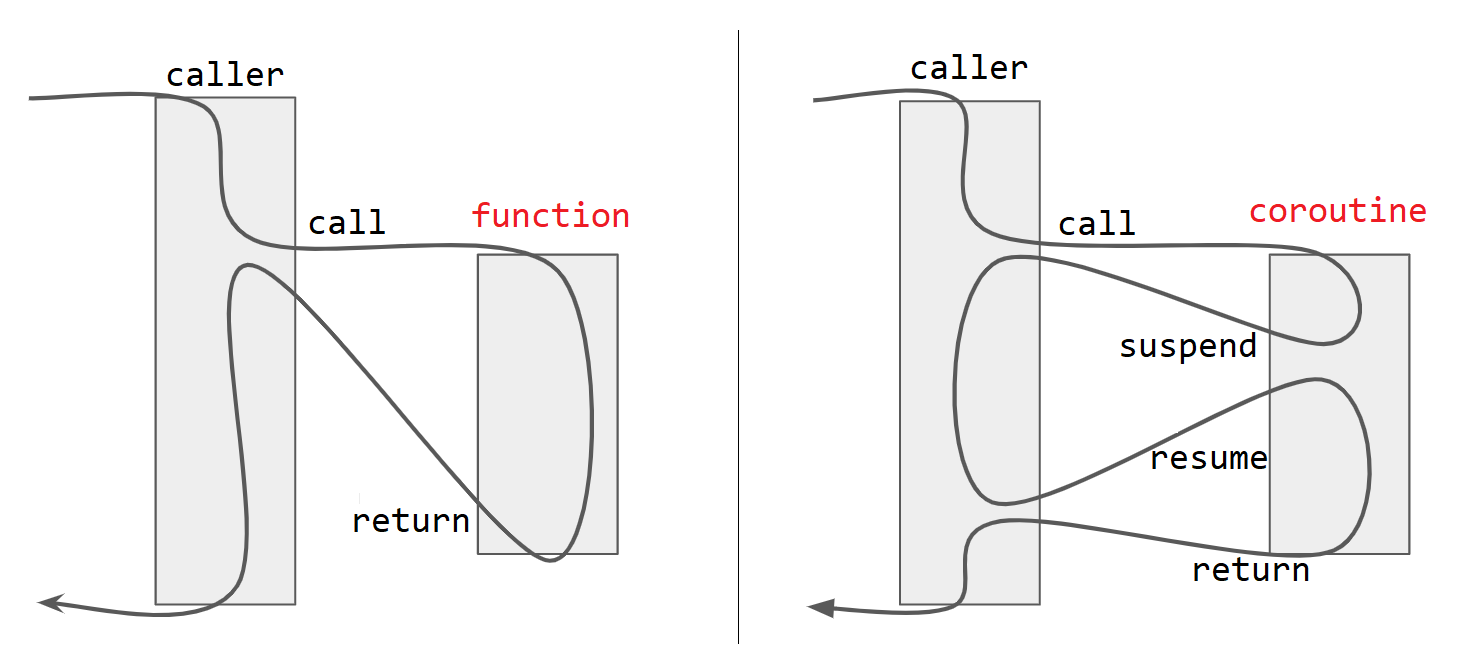
\includegraphics[width=1\textwidth, height=1\textheight, keepaspectratio]{./imgs/C++20-Coroutine.png}
	\caption{C++20 Coroutines}
	\label{fig:coroutines}
\end{figure}

\subsubsection{Terminologia delle Coroutine}

\textsf{\small \textbf{Awaitable}} \\

\begin{itemize}
	\item \textsf{\small È un tipo che supporta l'operatore \emph{co\_await}.}
	%\item \textsf{\small }
\end{itemize}

\begin{lstlisting}
	class dummy { // Awaitable
		public:
			std::suspend_always operator co_await(){ return {}; }
	};

	HelloWorldCoro print_hello_world() 
	{
		std::cout << "Hello ";
		co_await dummy{}; 
		std::cout << "World!" << std::endl;
	}
\end{lstlisting}

\textsf{\small \textbf{Awaiter}} \\

\begin{itemize}
	\item \textsf{\small È un tipo che implementa tre speciali funzioni che sono chiamate come parte dell'espressione \emph{co\_await}: \emph{await\_ready()}, \emph{await\_suspend()}, \emph{await\_resume()}. Per esempio, la \emph{Libreria Standard} ha definito degli \emph{awaiters}: \emph{std::suspend\_always} e \emph{std::suspend\_never}.}
	\item \textsf{\small Un tipo può essere sia di tipo \textbf{Awaitable} che \textbf{Awaiter}.}
\end{itemize}

\begin{lstlisting}
	class MyAwaiter {
		public:
			bool await_ready() { return false; } 
			void await_suspend(std::coroutine_handle<>) {} 
			void await_resume() {}
	};
	
	HelloWorldCoro print_hello_world() 
	{
		std::cout << "Hello ";
		co_await MyAwaiter{};
		std::cout << "World!" << std::endl;
	}
\end{lstlisting}

\textsf{\small \textbf{co\_await}: } \\

\begin{itemize}
	\item \textsf{\small è un operatore unario che sospende la \textbf{coroutine} e restituisce il controllo al chiamante. Il suo operando è una espressione il cui l'operatore deve definire \textbf{co\_await} o \textbf{Awaitable}.}
\end{itemize}

\begin{lstlisting}
	class dummy { }; // Awaitable
	
	class HelloWorldCoro {
		public:
			class promise_type {
				public:
					// . . .
					auto await_transform(const dummy&) 
					{
						return std::suspend_always{};
					}
			};
			// . . .
	};
	
	HelloWorldCoro print_hello_world() {
		std::cout << "Hello ";
		co_await dummy{}; 
		std::cout << "World!" << std::endl;
	}
\end{lstlisting}

\textsf{\small \textbf{Promise}: } \\

\begin{itemize}
	\item \textsf{\small Un tipo strettamente chiamato \emph{promise\_type}.}
	\item \textsf{\small È usato dentro al \textbf{coroutine}. La \textbf{coroutine} sottomette il proprio risultato o eccezione attraverso questo oggetto.}
	\item \textsf{\small La tipologia del \emph{promise type} è determinato dal compilatore dal tipo di ritorno del \textbf{coroutine} usando \emph{std::coroutine\_traits}.}
\end{itemize}

\textsf{\small \textbf{Coroutine Handle}: } \\

\begin{itemize}
	\item \textsf{\small È usato per riprendere l'esecuzione della \textbf{coroutine} o per distruggerla. Indica anche lo stato della \textbf{coroutine} usando \emph{std::coroutine\_handle::done()}.}
\end{itemize}

\textsf{\small \textbf{Coroutine State}: } \\

\begin{itemize}
	\item \textsf{\small È un oggetto generato dal compilatore, memorizzato sull'heap che contiene: }
	\begin{itemize}
		\item \textsf{\small L'oggetto \emph{promise} (promessa).}
		\item \textsf{\small I parametri (tutti copiati per valore).}
		\item \textsf{\small Le variabili locali.}
		\item \textsf{\small La rappresentazione del punto di sospensione attuale, così che la \emph{resume} sappia da dove continuare e la destroy sa quali variabili si trovano nello scope (nella portata).}
	\end{itemize}
\end{itemize}

\subsubsection{Esempi di coroutines}

\textsf{\small Per usufruire delle \textbf{coroutines} è necessario includere \textbf{<coroutine>}.} \break

\textsf{\small Sospendere una \textbf{coroutine}: } \\

\begin{lstlisting}
	// Flags compilatore: -std=c++20 -fcoroutines -fno-exceptions
	#include <iostream>
	#include <coroutine>
	
	class HelloWorldCoro {
		public:
		class promise_type { // compiler looks for `promise\_type`
			public:
			HelloWorldCoro get_return_object() { return this; }    
			std::suspend_always initial_suspend() { return {}; }        
			std::suspend_always final_suspend() { return {}; }
		};
		
		HelloWorldCoro(promise_type* p) : m_handle(std::coroutine_handle<promise_type>::from_promise(*p)) {}
		~HelloWorldCoro() { m_handle.destroy(); }
		
		std::coroutine_handle<promise_type>      m_handle;
	};
	
	HelloWorldCoro print_hello_world() {
		std::cout << "Hello ";
		co_await std::suspend_always{};
		std::cout << "World!" << std::endl;
	}
	
	int main() {
		HelloWorldCoro mycoro = print_hello_world();
		
		mycoro.m_handle.resume();
		mycoro.m_handle(); // Equal to mycoro.m\_handle.resume();
		return EXIT_SUCCESS;
	}
\end{lstlisting}

\textsf{\small Una \textbf{coroutine} può essere ripresa da una funzione membro del \emph{std::coroutine\_handle} o invocando la funzione operatore dell'oggetto \emph{std::coroutine\_handle}.} \\

\textsf{\small Come detto in precedenza, la \textbf{coroutine} consiste in: } \\

\begin{itemize}
	\item \textsf{\small La \emph{promessa}, nel nostro esempio \emph{promise\_type}.}
	\item \textsf{\small \emph{Awaiter}, nel nostro esempio \emph{std::suspend\_always}.}
	\item \textsf{\small \emph{Coroutine Handle}, nel nostro esempio \emph{std::coroutine\_handle}.}
\end{itemize}

%\textsf{\small } \\

\textsf{\small Restituire un valore dalla \textbf{coroutine}: } \\

\begin{lstlisting}
	// Flags compilatore: -std=c++20 -fcoroutines -fno-exceptions
	#include <iostream>
	#include <coroutine>
	#include <cassert>
	
	class HelloWorldCoro {
		public:
		class promise_type {
			public:
			int m_value;
			
			HelloWorldCoro get_return_object() { return this; }
			std::suspend_always initial_suspend() { return {}; }
			std::suspend_always final_suspend() { return {}; }
			
			void return_value(int val) { m_value = val; }
		};
		
		HelloWorldCoro(promise_type* p) : m_handle(std::coroutine_handle<promise_type>::from_promise(*p)) {}
		~HelloWorldCoro() { m_handle.destroy(); }
		
		std::coroutine_handle<promise_type>      m_handle;
	};
	
	HelloWorldCoro print_hello_world() {
		std::cout << "Hello ";
		co_await std::suspend_always{ };
		std::cout << "World!" << std::endl;
		
		co_return -1;
	}
	
	
	int main() {
		HelloWorldCoro mycoro = print_hello_world();
		
		mycoro.m_handle.resume();
		mycoro.m_handle.resume();
		assert(mycoro.m_handle.promise().m_value == -1);
		
		//Output: Hello World!
		
		return EXIT_SUCCESS;
	}
\end{lstlisting}

\textsf{\small Per restituire un valore dalla \textbf{coroutine}, c'è bisogno di fornire la funzione \emph{return\_value} al \emph{promise type}.} \\

\textsf{\small Rendere (\emph{Yielding}) un valore dalle \textbf{coroutines}: } \\

\begin{lstlisting}
	// Flags compilatore: -std=c++20 -fcoroutines -fno-exceptions
	#include <iostream>
	#include <coroutine>
	#include <cassert>
	
	class HelloWorldCoro {
		public:
		class promise_type {
			public:
			int m_val;
			
			HelloWorldCoro get_return_object() { return this; } 
			std::suspend_always initial_suspend() { return {}; } 
			std::suspend_always final_suspend() { return {}; } 
			
			std::suspend_always yield_value(int val) {
				m_val = val; 
				return {};
			}
		};
		
		HelloWorldCoro(promise_type* p) : m_handle(std::coroutine_handle<promise_type>::from_promise(*p)) {}
		~HelloWorldCoro() { m_handle.destroy(); }
		
		std::coroutine_handle<promise_type>      m_handle;
	};
	
	HelloWorldCoro print_hello_world() {
		std::cout << "Hello ";
		co_yield 1;
		std::cout << "World!" << std::endl;
	}
	
	int main() {
		HelloWorldCoro mycoro = print_hello_world();
		
		mycoro.m_handle.resume();
		assert(mycoro.m_handle.promise().m_val == 1);
		mycoro.m_handle.resume();
		
		//Output: Hello World!
		return EXIT_SUCCESS;
	}
\end{lstlisting}

\textsf{\small Per poter rendere, produrre (\emph{yielding}) un valore dalla \textbf{coroutine} è necessario fornire la funzione \emph{yield\_value()} al \emph{promise\_type} che restituisce il \emph{awaitable\_type}. } \\

\textsf{\small Generando una sequenza di numeri interi con le \textbf{coroutine}: } \\

\begin{lstlisting}
	// Flags compilatore: -std=c++20 -fcoroutines -fno-exceptions
	#include <iostream>
	#include <coroutine>
	
	class Generator {
		public:
		class promise_type {
			public:
			int m_val;
			
			Generator get_return_object() { return this; }
			std::suspend_never initial_suspend() { return {}; }
			std::suspend_always final_suspend() { return {}; }
			
			std::suspend_always yield_value(int val) {
				m_val = val; 
				return {};
			}
		};
		
		class iterator {
			public:
			bool operator!=(const iterator& rhs) { return not m_h_ptr->done(); }
			iterator& operator++() { 
				m_h_ptr->resume(); 
				return *this; 
			}
			int operator*() { return m_h_ptr->promise().m_val; }
			
			std::coroutine_handle<promise_type> *m_h_ptr;
		};
		
		iterator begin() { return iterator{&m_handle}; }
		iterator end() { return iterator{nullptr}; }
		
		Generator(promise_type* p) : m_handle(std::coroutine_handle<promise_type>::from_promise(*p)) {}
		~Generator() { m_handle.destroy(); }
		
		std::coroutine_handle<promise_type>      m_handle;
	};
	
	
	Generator range(uint32_t start, uint32_t end) {
		while(start != end)
		co_yield start++;
	}
	
	int main() {
		for (auto &&no : range(0, 10)) { 
			std::cout<< no <<std::endl;
		}
		//Output: 0
		//Output: 1
		//Output: 2
		//Output: 3
		//Output: 4
		//Output: 5
		//Output: 6
		//Output: 7
		//Output: 8
		//Output: 9
		
		return EXIT_SUCCESS;
	}
\end{lstlisting}

\textsf{\small Questo è in breve cosa sono e a cosa servono le \textbf{coroutines} del \textbf{C++20}, anche qui si potrebbe estendere e approfondire l'argomento, ma per il momento vediamo soltanto un piccolo assaggio. } \\

\subsubsection{Stackfull \& Stackless Coroutines}

\textsf{\small Cosa sono le \textbf{stackfull} e le \textbf{stackless coroutines}?} \\

\begin{itemize}
	\item \textsf{\small \textbf{Stackfull} : Le \textbf{stackfull coroutines} hanno bisogno di uno \emph{stack} separato per essere eseguite.}
	\item \textsf{\small \textbf{Stackless} : Le \textbf{stackless coroutines} usano lo stesso \emph{stack} del chiamante.}
\end{itemize}

\subsubsection{Differenza tra threads vs coroutines}

\begin{itemize}
	\item \textsf{\small Le \textbf{coroutines} riguardano il \emph{programming model} (modello di programmazione) mentre le \textbf{threads} riguardano l'\emph{execution model} (modello d'esecuzione).} \\
	\item \textsf{\small Le \textbf{coroutines} possono ancora fare \emph{concorrenza} senza l'\emph{overhead} (sovraccarico) dello scheduler, semplicemente gestisce lo \emph{context-switching} stesso.} \\
	\item \textsf{\small Un altro beneficio delle \textbf{coroutine} è il loro minore uso di memoria. Con i \textbf{thread}, ognuno di essi ha bisogno di allocare il proprio \emph{stack} e così la memoria cresce linearmente, mentre il numero di \textbf{coroutines} non ha una relazione diretta con l'utilizzo di memoria. } \\
\end{itemize}

\break

\textsf{\small Queste sono le \emph{4 Big} \emph{features} del \textbf{C++20} che cambieranno il modo di scrivere C++.} \\

\textsf{\small Le abbiamo soltanto trattate in modo breve e coinciso, ma sono 4 argomenti fondamentali del \textbf{C++20}.} \\

% ------------------------------ FINE CAPITOLO ---------------------------------------